% !TeX encoding = UTF-8

% 载入 SJTUThesis 模版
\documentclass[type=master, openany]{sjtuthesis}
% 选项
%   type=[doctor|master|bachelor],     % 可选(默认:master),论文类型
%   zihao=[-4|5],                      % 可选(默认:-4),正文字号大小
%   lang=[zh|en|de|ja],                % 可选(默认:zh),论文的主要语言
%   review,                            % 可选(默认:关闭),盲审模式
%   [twoside|oneside],                 % 可选(默认:twoside),双页或单页边距模式
%   [openright|openany],               % 可选(默认:openright),奇数页或任意页开始新章
%   math-style=[ISO|TeX],              % 可选 (默认:ISO),数学符号样式

% 论文基本配置,加载宏包等全局配置
% !TEX root = ./main.tex

\sjtusetup{
  %
  %******************************
  % 注意:
  %   1. 配置里面不要出现空行
  %   2. 不需要的配置信息可以删除
  %******************************
  %
  % 信息录入
  %
  info = {%
    %
    % 标题
    %
    zh / title           = {基于静态单赋值中间语言的函数式编译器\\ 验证方法},
    en / title           = {Verification of Functional Compilers Based on Static Single Assignment Intermediate Representation},
    %
    % 标题页标题
    %   可使用“\\”命令手动控制换行
    % 
    % zh / display-title   = {上海交通大学学位论文\\ \LaTeX{} 模板示例文档},
    % en / display-title   = {A Sample Document \\ for \LaTeX-based SJTU Thesis Template},
    %
    % 关键词
    %
    zh / keywords        = {编译器验证, 形式化方法, 静态单赋值, 函数式编译器},
    en / keywords        = {Compiler Verification, Formal Methods, Static Single Assignment, Functional Compilers},
    %
    % 姓名
    %
    zh / author          = {刘思雨},
    en / author          = {Siyu Liu},
    %
    % 指导教师
    %
    zh / supervisor      = {汪宇霆副教授},
    en / supervisor      = {Assoc. Prof. Yuting Wang},
    %
    % 副指导教师
    %
    % assoc-supervisor  = {某某教授},
    % assoc-supervisor* = {Prof. Uom Uom},
    %
    % 学号
    %
    id              = {121033910117},
    %
    % 学位
    %   本科生不需要填写
    %
    zh / degree          = {专业学位硕士},
    en / degree          = {Master of Engineering},
    %
    % 专业
    %
    zh / major           = {计算机技术},
    en / major           = {Computer Technology},
    %
    % 所属院系
    %
    zh / department      = {计算机科学与工程系},
    en / department      = {Department of Computer Science and Engineering},
    %
    % 答辩日期
    %   使用 ISO 格式 (yyyy-mm-dd);默认为当前时间
    %
    % date                 = {2023-05-18},
    %
    % 标题页显示日期
    %   覆盖对应标题页的日期显示,原样输出
    %
    % zh / display-date    = {2023 年 5 月},
    %
    % 资助基金
    %
    % zh / fund  = {
    %                {国家 973 项目 (No. 2025CB000000)},
    %                {国家自然科学基金 (No. 81120250000)},
    %              },
    % en / fund  = {
    %                {National Basic Research Program of China (Grant No. 2025CB000000)},
    %                {National Natural Science Foundation of China (Grant No. 81120250000)},
    %              },
  },
  %
  % 风格设置
  %
  style = {%
    %
    % 论文标题页 logo 颜色 (red/blue/black)
    %
    % title-logo-color = black,
  },
  %
  % 名称设置
  %
  name = {
    % bib             = {References},
    % ack             = {谢\hspace{\ccwd}辞},
    % achv            = {攻读学位期间完成的论文},
  },
}

% 使用 BibLaTeX 处理参考文献
%   biblatex-gb7714-2015 常用选项
%     gbnamefmt=lowercase     姓名大小写由输入信息确定
%     gbpub=false             禁用出版信息缺失处理
\usepackage[backend=biber,style=gb7714-2015]{biblatex}
% 文献表字体
% \renewcommand{\bibfont}{\zihao{5}\fixedlineskip{15.6bp}}
% 文献表条目间的间距
\setlength{\bibitemsep}{0pt}
% 导入参考文献数据库
\addbibresource{refs.bib}

% 脚注格式
\usepackage[perpage,bottom,hang]{footmisc}

% 定义图片文件目录与扩展名
\graphicspath{{figures/}}
\DeclareGraphicsExtensions{.pdf,.eps,.png,.jpg,.jpeg}

% 确定浮动对象的位置,可以使用 [H],强制将浮动对象放到这里(可能效果很差)
% \usepackage{float}

% 固定宽度的表格
% \usepackage{tabularx}

% 使用三线表:toprule,midrule,bottomrule。
\usepackage{booktabs}

% 表格中支持跨行
\usepackage{multirow}

% 表格中数字按小数点对齐
\usepackage{dcolumn}
\newcolumntype{d}[1]{D{.}{.}{#1}}

% 使用长表格
\usepackage{longtable}

% 附带脚注的表格
\usepackage{threeparttable}

% 附带脚注的长表格
\usepackage{threeparttablex}

% 算法环境宏包
\usepackage[ruled,vlined,linesnumbered]{algorithm2e}
% \usepackage{algorithm, algorithmicx, algpseudocode}

% 代码环境宏包
\usepackage{listings}
\usepackage{xcolor}
\definecolor{dkgreen}{rgb}{0,0.6,0}
\definecolor{ltblue}{rgb}{0,0.4,0.4}
\definecolor{dkviolet}{rgb}{0.3,0,0.5}
% lstlisting coq style (inspired from a file of Assia Mahboubi)
\lstdefinelanguage{Coq}{ 
    % Anything betweeen $ becomes LaTeX math mode
    mathescape=true,
    % Comments may or not include Latex commands
    texcl=false, 
    % Vernacular commands
    morekeywords=[1]{Section, Module, End, Require, Import, Export,
        Variable, Variables, Parameter, Parameters, Axiom, Hypothesis,
        Hypotheses, Notation, Local, Tactic, Reserved, Scope, Open, Close,
        Bind, Delimit, Definition, Let, Ltac, Fixpoint, CoFixpoint, Add,
        Morphism, Relation, Implicit, Arguments, Unset, Contextual,
        Strict, Prenex, Implicits, Inductive, CoInductive, Record,
        Structure, Canonical, Coercion, Context, Class, Global, Instance,
        Program, Infix, Theorem, Lemma, Corollary, Proposition, Fact,
        Remark, Example, Proof, Goal, Save, Qed, Defined, Hint, Resolve,
        Rewrite, View, Search, Show, Print, Printing, All, Eval, Check,
        Projections, inside, outside, Def},
    % Gallina
    morekeywords=[2]{forall, exists, exists2, fun, fix, cofix, struct,
        match, with, end, as, in, return, let, if, is, then, else, for, of,
        nosimpl, when},
    % Sorts
    morekeywords=[3]{Type, Prop, Set, true, false, option},
    % Various tactics, some are std Coq subsumed by ssr, for the manual purpose
    morekeywords=[4]{pose, set, move, case, elim, apply, clear, hnf,
        intro, intros, generalize, rename, pattern, after, destruct,
        induction, using, refine, inversion, injection, rewrite, congr,
        unlock, compute, ring, field, fourier, replace, fold, unfold,
        change, cutrewrite, simpl, have, suff, wlog, suffices, without,
        loss, nat_norm, assert, cut, trivial, revert, bool_congr, nat_congr,
        symmetry, transitivity, auto, split, left, right, autorewrite},
    % Terminators
    morekeywords=[5]{by, done, exact, reflexivity, tauto, romega, omega,
        assumption, solve, contradiction, discriminate},
    % Control
    morekeywords=[6]{do, last, first, try, idtac, repeat},
    % Comments delimiters, we do turn this off for the manual
    morecomment=[s]{(*}{*)},
    % Spaces are not displayed as a special character
    showstringspaces=false,
    % String delimiters
    morestring=[b]",
    morestring=[d]’,
    % Size of tabulations
    tabsize=3,
    % Enables ASCII chars 128 to 255
    extendedchars=false,
    % Case sensitivity
    sensitive=true,
    % Automatic breaking of long lines
    xleftmargin       = 1em,
    xrightmargin      = 1em,
    breaklines=false,
    framexleftmargin  = 1em,
    framexrightmargin = 1em,
    keepspaces        = true,
    backgroundcolor   = \color{gray!10},
    % Default style fors listings
    basicstyle=\normalsize,
    % numbers=left,
    % numberstyle=\small\color{gray},
    % Position of captions is bottom
    captionpos=b,
    % flexible columns
    columns=[l]flexible,
    % Style for (listings') identifiers
    identifierstyle={\ttfamily\color{black}},
    % Style for declaration keywords
    keywordstyle=[1]{\ttfamily\color{dkviolet}},
    % Style for gallina keywords
    keywordstyle=[2]{\ttfamily\color{dkgreen}},
    % Style for sorts keywords
    keywordstyle=[3]{\ttfamily\color{ltblue}},
    % Style for tactics keywords
    keywordstyle=[4]{\ttfamily\color{ltblue}},
    % Style for terminators keywords
    keywordstyle=[5]{\ttfamily\color{dkred}},
    %Style for iterators
    %keywordstyle=[6]{\ttfamily\color{dkpink}},
    % Style for strings
    stringstyle=\ttfamily,
    % Style for comments
    commentstyle={\ttfamily\color{dkgreen}},
    %moredelim=**[is][\ttfamily\color{red}]{/&}{&/},
    literate=
    {\\forall}{{\color{dkgreen}{$\forall\;$}}}1
    {\\exists}{{$\exists\;$}}1
    {<-}{{$\leftarrow\;$}}1
    {=>}{{$\Rightarrow\;$}}1
    {==}{{\code{==}\;}}1
    {==>}{{\code{==>}\;}}1
    %    {:>}{{\code{:>}\;}}1
    {->}{{$\rightarrow\;$}}1
    {<->}{{$\leftrightarrow\;$}}1
    {<==}{{$\leq\;$}}1
    {\#}{{$^\star$}}1 
    {\\o}{{$\circ\;$}}1 
    {\@}{{$\cdot$}}1 
    {\/\\}{{$\wedge\;$}}1
    {\\\/}{{$\vee\;$}}1
    {++}{{\code{++}}}1
    {~}{{$\sim$}}1
    {\@\@}{{$@$}}1
    {\\mapsto}{{$\mapsto\;$}}1
    {\\hline}{{\rule{\linewidth}{0.5pt}}}1
    %
}[keywords,comments,strings]
\lstdefinestyle{lstStyleCode}{%
  aboveskip         = \medskipamount,
  belowskip         = \medskipamount,
  basicstyle        = \ttfamily\zihao{6},
  commentstyle      = \slshape\color{black!60},
  stringstyle       = \color{green!40!black!100},
  keywordstyle      = \bfseries\color{blue!50!black},
  extendedchars     = false,
  upquote           = true,
  tabsize           = 2,
  showstringspaces  = false,
  xleftmargin       = 1em,
  xrightmargin      = 1em,
  breaklines        = false,
  framexleftmargin  = 1em,
  framexrightmargin = 1em,
  backgroundcolor   = \color{gray!10},
  columns           = flexible,
  keepspaces        = true,
  texcl             = true,
  mathescape        = true
}
\lstnewenvironment{codeblock}[1][]{%
  \lstset{style=lstStyleCode,#1}}{}
% 将lstlisting的名称修改为中文
\renewcommand\lstlistingname{图}

% 直立体数学符号
\providecommand{\dd}{\mathop{}\!\mathrm{d}}
\providecommand{\ee}{\mathrm{e}}
\providecommand{\ii}{\mathrm{i}}
\providecommand{\jj}{\mathrm{j}}

% 国际单位制宏包
\usepackage{siunitx}

% 定理环境宏包
\usepackage{ntheorem}
% \usepackage{amsthm}

% 绘图宏包
\usepackage{tikz}
\usetikzlibrary{arrows.meta, shapes.geometric, chains, shadows.blur}

% 一些文档中用到的 logo
\usepackage{hologo}
\providecommand{\XeTeX}{\hologo{XeTeX}}
\providecommand{\BibLaTeX}{\textsc{Bib}\LaTeX}

% 借用 ltxdoc 里面的几个命令方便写文档
\DeclareRobustCommand\cs[1]{\texttt{\char`\\#1}}
\providecommand\pkg[1]{{\sffamily#1}}

% hyperref 宏包在最后调用
\usepackage{hyperref}

% E-mail
\providecommand{\email}[1]{\href{mailto:#1}{\urlstyle{tt}\nolinkurl{#1}}}

% \usepackage{amssymb}
\usepackage{graphicx}
\usepackage[misc,geometry]{ifsym}
\usepackage{caption}
\usepackage{subcaption}
\usepackage{amsmath}
\usepackage{multicol}
\usepackage{multirow}
\usepackage{mathtools}
\usepackage{enumitem}
\usepackage{setspace}
\usepackage{fancyhdr}
\usepackage{etoolbox}
\usepackage{bm}
\usepackage{tabularray}

\newcommand\doubleplus{\mathbin{+\mkern-5mu+}}


\begin{document}

%TC:ignore

% 标题页
\maketitle

% 原创性声明及使用授权书
\copyrightpage
% 插入外置原创性声明及使用授权书
% 此时必须在导言区使用 \usepackage{pdfpages}
% \copyrightpage[scans/sample-copyright.pdf]

% 前置部分
\frontmatter

% 摘要
% !TEX root = ../main.tex

\begin{abstract}[zh]
  静态单赋值(Static Single Assignment, SSA)形式的中间语言(Intermediate Representation, IR)
  被现代主流编译器基础设施广泛采用。
  这是因为它能够实现许多基于数据流分析的编译优化,从而显著提高编译器的编译效率。
  现有的函数式编译器一般会将源程序编译为延续传递风格(Continuation Passing Style, CPS),
  以得到明确的控制流。
  函数式语言编译器如果想利用基于数据流分析的丰富优化,就需要将延续传递风格的程序与静态单赋值中间语言连接起来。
  编译器作为重要的系统软件,其正确性也一直是研究者们不断探讨的方向。
  随着形式化方法理论和工具的发展,编译器的形式化验证已经被证明是确保编译过程正确性的有效方法。

  本文研究了如何将关键的函数式语言编译过程与静态单赋值中间语言通过形式化方法联系起来,
  从而在确保编译正确性的情况下使函数式语言的编译器能够充分利用静态单赋值中间语言的优势。
  我们设计了从延续传递风格的函数式程序到静态单赋值中间语言的转换算法,
  并对该转换算法进行了基于模拟技术的形式化验证。
  建立了这样的联系,才能够使经验证的函数式编译器复用基于静态单赋值的程序分析与编译优化,
  从而使高可靠的函数式编译器得到效率提升。
  本文还以代表性的基础函数式编程语言PCF(Programming Computable Functions)为研究对象,
  应用该经验证的编译过程构建出了PCF语言到LLVM中间语言的函数式编译器。
  具体而言,我们首先读入直接风格的PCF源程序,将其转换为延续传递风格,再编译到静态单赋值中间语言。
  我们对这条编译链的正确性进行形式化验证,并将它与LLVM中间语言连接起来。
  该工作为构建经验证的高性能、高可靠函数式编译器提供了基础。
  本文涉及的所有转换算法和定理证明均在Coq定理证明器中实现。
\end{abstract}

\begin{abstract}[en]
  Intermediate Representation (IR) in Static Single Assignment (SSA) form
  has been widely adopted by modern mainstream compiler infrastructures.
  It facilitates numerous compilation optimizations based on data-flow analysis,
  so as to significantly improve the performance of compilers.
  Existing functional compilers often translate source programs into 
  Continuation Passing Style (CPS) to achieve explicit control flow. 
  To harness the improvement provided by optimizations based on data-flow analysis, 
  a functional compiler needs to establish a connection between 
  programs in CPS and the SSA IR. 
  As essential components of system software, correctness of compilers have been the 
  subject of continuous exploration by researchers.
  With the development of the theory and tools for formal methods, 
  the formal verification of compilers has proven to be an effective approach 
  in ensuring their correctness.
  
  This paper investigates how to formally connect the key processes 
  of functional language compilation with SSA intermediate language, 
  enabling functional language compilers to harness the advantages of SSA 
  while ensuring compilation correctness. 
  In this paper, we design a transformation algorithm from CPS functional programs 
  to SSA intermediate language and formally verify this transformation algorithm 
  using simulation methods. Establishing such a connection enables 
  verified functional compilers to leverage SSA-based program analysis 
  and compilation optimizations, thus enhancing the efficiency of 
  highly reliable compilers for functional languages. 
  Furthermore, this paper takes the representative foundational functional 
  programming language, PCF (Programming Computable Functions), 
  as the source language. Applying the verified compilation process, 
  we construct a functional compiler for translating PCF programs to 
  LLVM intermediate language. Specifically, it involves the initial transformation
  of the direct-style PCF source code into CPS, followed by compilation into the SSA. 
  We formally verify the correctness of this compilation chain and connect it to the LLVM IR. 
  It provides the foundation for constructing a verified, high-performance, 
  and highly reliable functional compiler. All the transformation algorithms and 
  proofs of theorem discussed in this paper have been implemented in the Coq theorem prover.
\end{abstract}


% 目录
\tableofcontents
% 插图索引
\listoffigures*
% 表格索引
\listoftables*
% 算法索引
\listofalgorithms*

% 符号对照表
% !TEX root = ../main.tex

\begin{nomenclature*}
\label{chap:symb}

\begin{longtable}{rl}
  $k$  & 延续变量  \\  
  $B$       & 可观察行为    \\
  $\mathcal{T}$  & 编译过程  \\
  $\sim$       & 程序状态之间的不变式    \\
  $M$  & 度量函数  \\
  $S$       & 程序状态    \\
  $\approx$       & 语义保存性质    \\
  $\Downarrow$  & 程序终止  \\
  $\Uparrow$       & 程序发散    \\
  $\rightarrow$  & 小步操作语义的一步转换  \\
  $\xrightarrow{+}$       & 小步操作语义的一步或多步转换    \\
  $\xrightarrow{*}$  & 小步操作语义的零步或一步或多步转换  \\
  $loc\; [x\mapsto v]$ & 把从$x$到$v$的映射添加到$loc$中  \\
  $\mathcal{F}_{proc}$  & CPS转换  \\
  $\mathcal{G}_{proc}$  & CPS到SSA的转换  \\
  $Comp$  & PCF到SSA的转换  \\
\end{longtable}

\end{nomenclature*}


%TC:endignore

% 主体部分
\mainmatter

% 正文内容
% !TEX root = ../main.tex

\chapter{绪论}


\section{引言}

编译器作为关键系统软件之一,其正确性对于计算机系统的安全运行有重要意义。
这是由于编译器可能在转换程序的过程中引入错误,导致目标程序的行为和源程序不一致,
进而使得在源程序端花费大量精力的测试和验证工作在目标程序层级失效。
虽然对于编译器一般会进行密集的测试,错误编译是小概率事件,但是这种偶发性的
由编译器引入的问题,对于安全关键系统而言是需要考虑的。
工业界长期以来对保障编译器正确性这个问题非常重视。例如,按照航空领域的RTCA DO178B/C标准~\cite{brosgol2010178c},
需要按照和机载软件一样的严格要求对待编译器。
对于庞大的编译器,通过测试找到它的错误其实是比较困难的。
编译器随机测试工具Csmith~\cite{csmith2011}已经发现了四百多个编译器错误,可见编译器中隐藏的风险数量之大。

编译器的形式化验证已被证实可以有效保证编译器的正确性,它从数学层面上确保了编译过程的正确性。
一个著名的例子是经过验证的C编译器CompCert~\cite{leroy2009formally},
它将C语言的一个有代表性的重要子集编译到了支持多种处理器架构的汇编代码(包括PowerPC、ARM、X86和RISC-V)。
其编译过程的正确性(即目标汇编程序保存了源C程序的语义)经过了形式化验证,并在Coq定理证明器中实现。

延续传递风格(Continuation-Passing Style, CPS)是一种函数式程序的中间语言(Intermediate Representation, IR),
它明确了函数式程序的控制流,从而为程序基于控制流的分析和优化提供了便利。
延续传递风格的中间语言在函数式程序的编译器中被
广泛采用\cite{belanger-cpp2013,dargaye2009verification,zoe-oopsla2021,zoe-icfp2021,wang-esop2016}。
然而,这也意味着经验证的函数式编译器不能直接得到主流编译器基础设施(例如LLVM和GCC)的支持。
这些主流编译器基础设施采用静态单赋值(Static Single Assignment, SSA)形式的中间语言。 
SSA中间语言在工业编译器中大大流行,因为它可以通过强制让每个变量只能被赋值一次来实现
便捷而准确的数据流分析(Data-Flow Analysis, DFA),进而实现各种基于数据流分析的激进优化。
许多流行的命令式编程语言(例如Rust~\cite{balasubramanian2017system}和Swift~\cite{zhang2012swift})
使用这些编译器基础设施作为其后端,生成性能优越的代码~\cite{lattner2006introduction}。
一些工业级的函数式编译器也开始采用SSA形式的中间语言。例如,SML-New Jersey的
新版本已经将其后端转向了LLVM~\cite{farvardin2020new}。

在本文中,我们研究了如何构建基于SSA中间语言的经验证的函数式语言编译器。
具体而言,我们设计并验证了从CPS到SSA的转换算法,以便在经验证的编译器领域中将
传统基于CPS的函数式编译器与基于SSA中间语言上工作的主流编译器后端连接起来。
尽管研究人员已经探讨了CPS和SSA程序结构之间的对应关系~\cite{appel1998ssa,ssabook},
和相互转换~\cite{farvardin2020new,kelsey1995correspondence},
但如何对转换算法进行形式化验证仍然是待解决的问题。

本文的主要贡献总结如下:

\begin{itemize}
    \item
    我们的主要贡献是设计和验证了从CPS到SSA的转换算法。该转换过程的源语言是代表性的
    函数式语言PCF\cite{plotkin1977lcf},我们首先需要将其转换为CPS形式。
    转换算法的SSA目标语言是LLVM IR的一种简化版本,保留了LLVM IR的基本结构。
    该转换是基于CPS和SSA结构上的对应关系设计的~\cite{appel1998ssa,kelsey1995correspondence}。
    我们为PCF和SSA语言定义了小步操作语义,使用基于模拟的方法证明目标程序实现了
    源程序的语义保存。据我们所知,这是第一个经过验证的从CPS函数式程序到SSA的转换。
    
    \item 
    我们还利用该经验证的编译链构建了PCF语言的编译器原型。它是部分经过形式化验证的,
    为未来构建更复杂更完整的经验证函数式语言编译器打下基础。
    具体而言,我们首先实现并验证了直接风格PCF语言的CPS转换,并将它连接到经验证的CPS到SSA的编译过程。
    然后,我们通过Vellvm提供的抽象语法(Vellvm是一个经过验证的LLVM基础设施~\cite{zakowski2021modular}),
    将SSA中间语言转换为LLVM IR。
    
\end{itemize}

在本章接下来的内容中,我们首先在\ref{sec:background}节介绍必要的相关背景知识,
并在\ref{sec:related}节讨论了领域内与本课题相关的工作。
在第\ref{ch:overview}章中,我们简要介绍了该部分经验证的PCF编译器原型。
我们在第\ref{ch:trans}章中讨论了CPS转换和CPS到SSA的转换算法设计,
并在第\ref{ch:verify}章中对该编译链进行形式化验证。
本文工作在Coq中的实现和评估将在第\ref{ch:implement}章中介绍。
最后,我们在第\ref{ch:summary}章中对本文内容进行总结。

\section{相关背景} \label{sec:background}

在本节中,我们将对该课题的相关背景进行介绍。
本文工作涉及函数式编程、编译器常用中间语言形式以及编译器形式化验证方法等方向。
首先,我们会介绍函数式编程的概念及其特性。
然后,我们将说明CPS形式是如何帮助函数式程序显式地表示控制流的,
并介绍了静态单赋值中间语言的相关特性以及CPS和SSA结构之间的对应关系。
接下来,我们介绍了在经验证的编译器CompCert中提出的基于模拟技术进行编译器验证的框架~\cite{leroy2009formally}。

\subsection{函数式编程}

函数式编程(Functional Programming)是一种通过应用和组合函数来构建程序的编程范式,
以$\lambda$演算($\lambda$-Calculus)作为其数学基础~\cite{church1985calculi}。
传统命令式编程中,计算通过执行程序语句序更新程序状态来实现。
相比之下,函数式编程中程序由包含函数定义和应用的表达式构成,而计算通过对表达式求值来实现。
函数式程序的一大特点是函数可以作为参数传递,或者被其他函数返回,形成所谓的高阶函数~\cite{sussman1998scheme}。
此外,纯粹函数式程序的执行不会引起改变程序状态的副作用。
这些特点使得函数式程序设计语言编写的程序更加简洁、安全和易于验证~\cite{hudak1989conception},
因此在并发编程、系统内存编程等方面获得了成功应用。

在学术界和工业界中,函数式编程的应用日趋广泛。
除了Haskell~\cite{o2008real}等纯函数式语言,OCaml、Erlang、Scala~\cite{cesarini2009erlang, odersky2014unifying}
等语言都对函数式编程有内生的支持,且诸多命令式编程语言如C++和Rust也在积极的引入函数式编程机制。
本文研究的函数式编程语言是学术界有广泛影响力的PCF(Programming Computable Functions)。
由于PCF可以看作是工业用函数式编程语言的核心,本文的研究结果可被推广至其他函数式语言。
关于PCF语言的更多特性将在第\ref{sec:cps}节中详述。

\subsection{延续传递风格与静态单赋值} \label{sec:bg_cpsssa}

函数式程序的形式有很多种,如直接风格(Direct Style)和延续传递风格(CPS)。
图~\ref{cpsdirect}展示了同样含义的函数式程序在这两种不同表示风格下的例子。
CPS的关键特性在于通过延续明确地表示程序的控制流。
CPS中的延续(Continuation)指的是当前执行节点后所有剩余计算的函数,
该函数需要把当前计算得到的结果作为其输入。
具体来说,CPS函数需要将延续作为额外的参数传入,
当运行该函数得到计算结果后,程序通过调用该延续来传递这个值,也就是``返回''该结果。
以图~\ref{fig:cps2}为例,函数$h$在CPS中的延续参数为$k$,在得到最终结果$z$之后,
程序调用$(k\; z)$以返回$z$,并执行$k$所代表的剩余计算。
当调用CPS函数时,调用者需要提供一个延续函数来表示剩余计算,且在CPS中所有中间结果、控制流中的控制点都需要被明确命名。
这些特点导致用户直接用CPS形式编写代码较为困难,但是由于明确表示的控制流利于程序分析和优化,
CPS是函数式语言编译器中常见的中间表示形式。

\begin{figure}
    % \vspace{-0.3cm}
    \centering
    \begin{subfigure}[b]{0.3\textwidth}
        \flushright
    % \small
     \begin{equation}
        \nonumber
        \begin{aligned}
        &  \mathbf{function}\; h(x,y) = \\
        & \quad (x*x)\; +\; (y*y) \\
        \end{aligned}
    \end{equation}
    \caption{Direct Style}
        \label{fig:ori2}
    \end{subfigure}
 %   \hfill
    \begin{subfigure}[b]{0.6\textwidth}
        \flushleft
        % \small
        \begin{equation}
            \nonumber
            \begin{aligned}
            & \mathbf{function}\; h(x,y,k)= \mathbf{let}\; x_1=x*x\; \mathbf{in} \\
            &  \quad   \mathbf{let}\; y_1=y*y\; \mathbf{in}\; (\mathbf{let}\; z=x_1+y_1\; \mathbf{in}\; (k\; z)) \\
            \end{aligned}
        \end{equation}
        \caption{CPS}
        \label{fig:cps2}
    \end{subfigure}
    \caption{直接风格和CPS形式的示例函数式程序}\label{cpsdirect}
  \end{figure}

Plotkin~\cite{plotkin1977lcf}、Danvy和Nielsen\cite{danvy2007one}等人研究了将直接风格的函数式程序转换为CPS程序的方法。
其中Plotkin的方法需要后续进行管理性缩减(Administrative Reduction),以去除冗余的$\lambda$结构。
Felleisen等人提出了另一种方法非组合式的方法,其基于$\lambda$-演算的语义。
Danvy和Nielsen将这两种方法联系起来,可以只通过一步转换完成,不需要在后续过程中进行管理性缩减。

静态单赋值(SSA)是命令式语言编译器中一种广泛使用的中间语言类型。
在SSA中,每个变量只能在一处被赋值,且被使用之前必须已经被赋值。
这种性质很接近函数式语言中的名字绑定(Name Binding)~\cite{ssabook}。
变量被划分为不同的版本,新版本的变量往往使用原名加下标来表示,以使每个定义得到自己的版本。
$\phi$节点($\phi$-nodes)作为特殊的程序语句被插入到基本代码块的开头,
从而按照前驱基本块的名字生成新变量的赋值语句。
这样一来,变量的使用定义链(Use-def Chains)更加清晰,从而使许多编译器优化算法
在SSA中间语言上能够更好地实现,例如常量传播、无用代码消除、寄存器分配等~\cite{ssabook,kelsey1995correspondence}。
作为示例,图~\ref{ssacfg}展示了一个SSA程序的控制流图(Control-Flow Graph)。
其中,基本代码块$b_2$的前驱基本块可以是$b_1$或$b_2$本身。
不同的前驱基本块对变量$y$有不同的赋值,在$b_1$和$b_2$中变量$y$被赋予了不同版本的名称。
基本块$b_2$开头的$\phi$节点将$y_1$和$y_3$作为参数,根据执行时控制流的实际前驱基本块来
选择正确的版本赋值给新的变量$y_2$。

LLVM IR就是一种基于SSA的中间代码。它作为一种高层次的汇编语言,提供了编译系统的中间层,
使得不同语言可以相互连接起来,复用其后端优化~\cite{lattner2006introduction}。
除了LLVM,还有很多编译器是基于SSA的,例如GCC编译器的中间语言GIMPLE~\cite{callanan2007extending}、
面向微软.NET平台的即时编译中间语言CIL(Common Intermediate Language)~\cite{thai2003net}等。

\begin{figure}[htbp]
    \centering
    % \documentclass{article}
% \usepackage{tikz}
% \usetikzlibrary{chains,shadows.blur}

% \begin{document}
\begin{tikzpicture}[auto,
%   node distance = 12mm,
%   start chain = going right,
  box/.style = {draw,rounded corners,blur shadow,fill=white,
        align=center}]
 \small
 \node[box] (b1) at(0,0)    {$v_1 \leftarrow 1$\\ 
                    $z_1 \leftarrow 8$ \\ 
                    $y_1 \leftarrow 4$};      
 \node[box] (b2) at(3,0)    {$y_2 \leftarrow \phi(y_1,y_3)$\\
                    $x_1 \leftarrow 5 + y_2$ \\
                    $y_3 \leftarrow x_1 * z_1$ \\
                    $x_2 \leftarrow x_1 - 1$ \\
                    $\mathbf{if}\; x_2 = 0$};      
 \node[box] (b3) at(6.5,0)    {$w_1 \leftarrow v_1 +y_3$\\ 
                    $\mathbf{return}\; w_1$};  
 \node at(4.0,1.5) {false};
 \node at(4.8,0.3) {true};

 \coordinate (b1n) at ([yshift=-31] b1);
 \coordinate (b2n) at ([yshift=-43] b2);
 \coordinate (b3n) at ([yshift=-25] b3);

 \node at (b1n)  {$b_1$};
 \node at (b2n)  {$b_2$};
 \node at (b3n)  {$b_3$};
 
 \begin{scope}[rounded corners,-latex]
  \path (b2.60) edge[bend right=50] (b2.120)
        (b1) edge (b2) (b2) edge (b3) ;
%   \draw (b3.230) -- ++(0,-0.3) -| ([xshift=-5mm]b2.west) |-
%   ([yshift=3mm]b2.130) -- (b2.130);
 \end{scope}
\end{tikzpicture}
% \end{document}      
    \caption{SSA程序的控制流图示例}\label{ssacfg}
\end{figure}

Appel等人~\cite{appel1998ssa}发现SSA也是一种函数式语言:$\lambda$演算和SSA虽然有不同的形式,
但它们所做的工作其实是相同的。L. Beringer~\cite{ssabook}给出了SSA的函数式表示,
将SSA中的相关术语与函数式编程中的概念联系起来。
例如,函数式语言中的$let$绑定对应着SSA中的赋值、绑定变量的词法作用域对应着SSA中的可支配区域。
$let$绑定与变量定义点之间的对应关系还延续到了程序结构的其他方面。
与命令式语言中的返回地址或函数指针相似,延续指定了当前代码片段求值完成后程序下一步该如何执行。
SSA中的控制流图对应着函数式编程中的函数,虽然顶层延续的参数在控制流图中并不是明确可见的,
但它对应一个命令式调用中用来保存返回地址的地方。
Kelsey~\cite{kelsey1995correspondence}通过将CPS中的$\lambda$进行标注来区分完整过程、跳转、延续,
进而将被这种标注的CPS程序转换为一种SSA程序。然而,Kelsey工作中的CPS和SSA语言与本文中所使用的差距较大。
Kelsey的CPS语言将二元表达式的参数和条件语句中的条件视为表达式,使其更类似于带有延续元素的标准函数式程序。
例如,在Kelsey的工作中,表达式$k; ((x+y)+z)$是允许的,但在我们的工作中,
它必须转换为$\mathbf{letop}; x_0 = x+y; \mathbf{in}; (\mathbf{letop}; x_1 = x_0+z; \mathbf{in}; k; x_1)$。
此外,Kelsey的转换算法选择先合并CPS过程,然后再将其作为整体进行转换。
因此,SSA程序的顶层单元是一整个过程,没有函数调用,这与本文中使用的基于LLVM IR的SSA语言不同。

\subsection{编译器形式化验证} \label{sec:compcertbackend}

我们使用CompCert~\cite{leroy2009formally}基于模拟(Simulation)技术的形式化验证框架来证明转换过程的正确性。
经过形式化验证的C语言子集编译器CompCert是由INRIA的Xavier Leroy领导开发的,在Coq定理证明工具中实现。

CompCert已被应用于诸如核电站控制软件和飞行控制系统的开发。
清华大学王生原、尚书等人设计并实现了基于CompCert的L2C编译器~\cite{shang2017key},被用于安全关键的工业领域。
L2C的源语言是被广泛用于安全关键的工业领域(高铁、核电站等)的 Lustre,
这些类型的应用对开发工具本身的安全性要求很高。它的目标语言是ComperCert中使用的C子集Clight。
南京大学冯新宇等人针对并发程序进行了单独编译验证~\cite{jiang2019towards}。他们提出了独立于语言的验证框架,
将顺序程序与无竞赛并发程序编译器验证工作联系起来,从而使针对顺序程序的编译器验证工作可以被重用。
使用这种框架,他们建立了CASCompCert。它扩展了ComperCert,可以对无竞赛Clight并发程序的单独编译进行验证,
且允许将并发Clight模块与包含良性竞赛的同步原语的x86-TSO实现进行连接。

CompCert提供了一套基于模拟技术验证编译过程正确性的理论和框架。该框架将编译过程的正确性定义为
语义保存性质(Semantic Preservation Property),即目标程序的行为应该与源程序的行为一致。
我们将程序的行为(Behaviors)描述为由小步操作语义(Small-Step Operational Semantics)生成的轨迹(Trace),
以便直接推导出编译器的正确性证明。根据CompCert中对语义保存性质的讨论,
通过为安全的源程序建立后向模拟(Backward Simulaion),可以证明语义保存性质。

接下来,我们会介绍一些概念来说明什么是安全程序的后向模拟。
可以通过程序语言的语义将可观察行为(Observable Behaviors)与程序关联起来。
程序的可观察行为可以分为终止(Termination)、发散(Divergence)和出错(Going wrong)。
如果用$P_1$表示源程序,$B$表示可观察行为,那么$P_1 \Downarrow B$表示执行程序$P_1$获得的可观察行为为$B$。
同样的表示方法也可以应用于目标程序。在CompCert框架中,仅对不会出错的安全的源程序提供正确性保证。
如果我们将编译过程表示为$\mathcal{T}$函数,则经过转换得到的目标程序可以表示为$\mathcal{T}(P_1)$。
编译安全程序的正确性可以描述为目标程序的行为是可接受的源程序行为。
那么,安全源程序的后向模拟可以表示为:如果$P_1$是一个安全程序,
则对于所有的可观察行为$B$,$\mathcal{T}(P_1) \Downarrow B \Longrightarrow P_1 \Downarrow B$。

然而,直接证明后向模拟是比较困难的。可以先建立从安全源程序到目标程序的前向模拟(Forward Simulation),
再根据目标程序的确定性和前向模拟来推导出后向模拟。
安全源程序的前向模拟可以表示为:如果$P_1$是一个安全程序,则对于所有的$B$,
$P_1 \Downarrow B \Longrightarrow \mathcal{T}(P_1) \Downarrow B$。
由于目标程序是确定性的(Deterministic),它只与一种行为相关联。
因此,目标程序不会具有$P_1$没有的额外行为。在这种情况下,可以从前向模拟中导出安全程序的后向模拟。

为了证明源语言$L_1$转换为目标语言$L_2$的编译过程满足前向模拟性质,
关键在于建立程序状态$S_1$和$S_2$之间的不变式(Invariant)$S_1\sim S_2$,
并证明它在源程序和目标程序的执行过程中始终成立。
按照CompCert的方法,我们首先需要为$L_1$和$L_2$定义操作语义。
对于任何源程序$P_1$和目标程序$P_2$,我们需要证明$P_1$和$P_2$的初始状态满足不变量$\sim$。
然后,我们需要证明它们的内部执行步骤始终可以通过$\sim$相关联。
也就是说,假设$S_1\sim S_2$,源程序的状态在一步执行后从$S_1$转换到$S'_1$,
那么目标程序状态从$S_2$转换到某个$S'_2$,需要保证在转换后$S'_1\sim S'_2$成立。
根据从$S_2$到$S'_2$的转换步骤数量,可以将模拟图(Simulation Diagram)分为以下几种:

\begin{figure}[ht]
    % \vspace{-10pt}
    \centering
    \begin{subfigure}[b]{0.26\textwidth}
        % \flushleft
        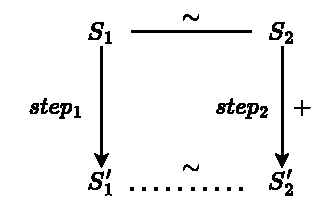
\includegraphics[width=1\linewidth]{figures/plusstep.pdf}
        \caption{多步模拟}
        \label{fig:plus}
    \end{subfigure}
    \begin{subfigure}[b]{0.52\textwidth}
        % \flushright
        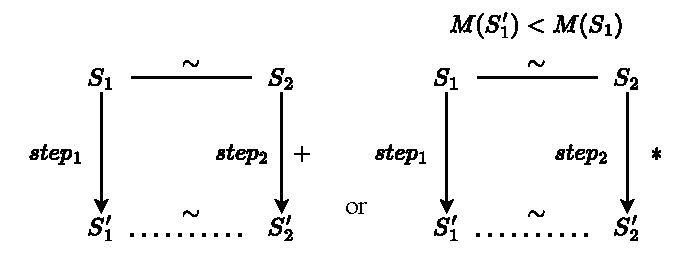
\includegraphics[width=1\linewidth]{figures/starstep2.pdf}
        \caption{星形模拟}
        \label{fig:star}
    \end{subfigure}
    \caption{不同类型的模拟图}\label{simustep}
\end{figure}

\begin{itemize}
    \item 一步模拟(Lock-Step Simulation)表示$S_2$经过一步转换到达$S'_2$状态。
        然而,对于大多数转换算法来说,一步模拟的前提要求太严格了,我们需要对其进行放宽。
    \item 多步模拟(Plus Simulation)表示$S_2$经过一步或多步转换到达$S'_2$(如图~\ref{fig:plus})。
        有时,从$S_1$到$S'_1$的转换对于状态$S_2$没有任何影响,比如删除冗余代码。
        因此,在某些情况下,多步模拟的条件也需要放松。
    \item 星形模拟(Star Simulation)表示$S_2$经过零步或一步或多步转换到达$S'_2$状态(如图~\ref{fig:star})。
        在这种条件下,可能会出现一种违反语义保存性质的情况:源程序发散,而目标程序保持在$S_2$状态,
        它们之间的状态仍然始终满足$\sim$不变式。为了防止出现这种``无限驻留''问题,我们需要
        为源程序的状态定义一个度量函数$M$,它随着源程序的执行过程严格减小。
        增添了度量函数$M$相关的限制,我们就能通过模拟保存源程序的发散行为了。
\end{itemize}

正如我们将在第~\ref{ch:verify}章中讨论的那样,CPS转换的前向模拟满足多步模拟性质,
而对于CPS到SSA的转换,我们需要使用星形模拟。根据上述模拟图性质以及
源程序和目标程序初始状态的对应关系,我们可以推导出安全程序的前向模拟。
结合目标语言的确定性,即可推导出安全程序的后向模拟。

由于语义保存性质是可传递的(Transitively Composable),
我们可以先分别证明各个编译过程的语义保存性质,然后将结果组合起来推导出整个编译过程的正确性。
例如,如果编译过程$\mathcal{T}$被分解为两个转换阶段$\mathcal{T}_1$和$\mathcal{T}_2$,
$\mathcal{T}$可以被视为它们的组合。对于一个安全的程序$P$,如果没有发生编译时错误(Compiler-Time Error),
$\mathcal{T}(P) = \mathcal{T}_2(\mathcal{T}_1(P))$。
如果我们可以验证$\mathcal{T}_1$和$\mathcal{T}_2$的正确性,那么$\mathcal{T}$也得到了验证。

\section{相关工作} \label{sec:related}

在编译器验证领域,许多工作是围绕CompCert编译器展开的,包括很多函数式语言编译器的验证工作。
例如,经验证的函数式编译器CertiCoq将Gallina(Coq语言)编译到了CompCert中使用的的Clight~\cite{belanger2019certified}。
miniML经验证的编译器也使用了CompCert框架,将其编译到了CompCert中的中间语言Cminor~\cite{dargaye2009verification}。
基于SSA的中间语言(例如LLVM IR)模块化、可移植和优化潜能大等特性引起了函数式编译器开发者的关注。
近年来,一些原本不使用SSA后端的函数式编译器已经开始转向SSA后端以获得更好的性能~\cite{farvardin2020new}。
我们的工作基于这些观察建立,是朝着构建利用SSA中间语言优势的经验证的函数式编译器迈出的第一步。

\subsection{Gallina经验证的编译器CertiCoq}

CertiCoq将Gallina编译到了C语言的子集Clight,以便与CompCert链接起来并最终编译到汇编语言,
从而获得一个完整的经过验证的编译链~\cite{belanger2019certified,zoe-oopsla2021,zoe-icfp2021}。
从CPS到Clight的编译过程及其形式化证明在Coq中实现,不过其使用的是大步操作语义而不是小步操作语义。
该编译器的目标语言不是基于SSA的,因此不能直接连接到LLVM框架,也不能利用基于SSA中间语言的优化。

\subsection{miniML经验证的编译器前端MLCompCert}

MLCompCert是Zaynah Dargaye等人设计的一个经验证的编译器前端~\cite{dargaye2009verification}。
它的源语言是ML纯函数式语言的部分,即miniML,包括了$\lambda$演算、$let$绑定、模式匹配等。
它的目标语言是CompCert编译器后端的中间语言Cminor,即一种类似于C语言的底层语言。
该编译器实现了一些经典的函数式程序编译优化,例如反柯里化(uncurrying)和统一数据结构表示等。
设计者们在Coq中对该函数式程序编译器前端进行了实现和验证。

\subsection{SML-New Jersey基于LLVM编译器后端的版本}

SML-New Jersey编译器(SML/NJ)是Standard ML的著名编译器。在最近发布的新版本中,它更改了后端,
将CPS中间语言编译到了LLVM IR~\cite{farvardin2020new}。CPS程序首先被转换为控制流图(Control-Flow Graph, CFG)中间语言,
然后再转换为LLVM IR。这是因为将CPS中间语言连接到基于SSA的编译器基础设施能够利用这些编译器提供的丰富后端优化。
但这项工作不是经过形式化验证的。
我们的工作受到了这一趋势的启发,并进一步尝试对这种连接进行形式化验证。

\subsection{CompCert支持SSA的扩展CompCertSSA}

经验证的编译器也开始试着支持基于SSA中间语言的后端了。
CompCertSSA是CompCert的一个扩展,具有一个基于SSA的中间端~\cite{compcertssa}。
它将SSA作为一种可选的优化中间语言,允许在RTL(Register Transfer Language)三地址代码和SSA中间语言之间进行转换。
虽然这使得CompCert能够实现一些基于SSA的优化~\cite{compcertssa-op,blazy-cpp2023},
但是CompCertSSA提供的优化仍然比较有限,不能与LLVM的后端优化相媲美。
不过,它提供了一个从C语言开始的经过完整验证的编译链,是开发针对SSA的经验证的函数式编译器的有力工具。

\subsection{经验证的LLVM IR: Vellvm}

Vellvm在定理证明工具Coq中定义了LLVM中间语言的抽象语法树(Abstract Syntax Tree, AST),并为LLVM IR提供了形式化语义。
早期版本的Vellvm提供了LLVM IR的操作语义~\cite{zhao2012formalizing},
而在较新版本中已迁移到了基于交互树(Interactive Tree, ITree)的语义~\cite{zakowski2021modular}。
在本文第\ref{ch:overview}章所介绍的编译链中,SSA程序首先被编译到了Vellvm AST,然后生成了最终的LLVM IR程序。

% !TEX root = ../main.tex

\chapter{相关工作与本文编译链概览} \label{ch:related}

如第\ref{sec:compcertbackend}节中所述,在经验证的编译器领域,许多工作是围绕CompCert编译器开展的。
我们将在第\ref{sec:relatedc}节中对CompCert及它的扩展CompCertSSA中端进行介绍。
在本章第\ref{sec:relatedf}节中,我们将对已有的针对函数式语言编译器的形式化验证工作进行介绍。
它们大部分还是基于CompCert完成的。 
国内外的研究者们已经注意到使函数式编译器复用基于SSA中间语言的基础设施后端的重要性。
在第\ref{sec:relatedssa}节中,我们对基于SSA中间语言的LLVM编译框架以及经验证的LLVM IR进行了介绍。
我们的工作基于对这些相关工作的观察建立,是朝着构建利用SSA中间语言优势的经验证的函数式编译器迈出的第一步。
我们构建了从PCF到SSA语言经验证的编译过程,并将其应用到目标语言是LLVM IR的编译链中。
在本章第~\ref{sec:overview}节中,我们对该编译链的每一步编译过程进行了简要介绍。

\section{经验证的编译器框架CompCert} \label{sec:relatedc}

经验证的C语言编译器CompCert提供了对编译器正确性进行形式化验证的理论和框架~\cite{leroy2009formally}。
它的大体编译流程如图\ref{fig:compcert}所示。该图是CompCert编译链图的简化版本,
省略了一些编译步骤,主要保留了我们在后文中介绍基于CompCert的工作时需要了解的中间语言和编译步骤。
本文中的工作所使用的基于模拟的验证技术是CompCert框架中提供的。
\begin{figure}[htbp]
    \centering
    \vspace{3ex}
    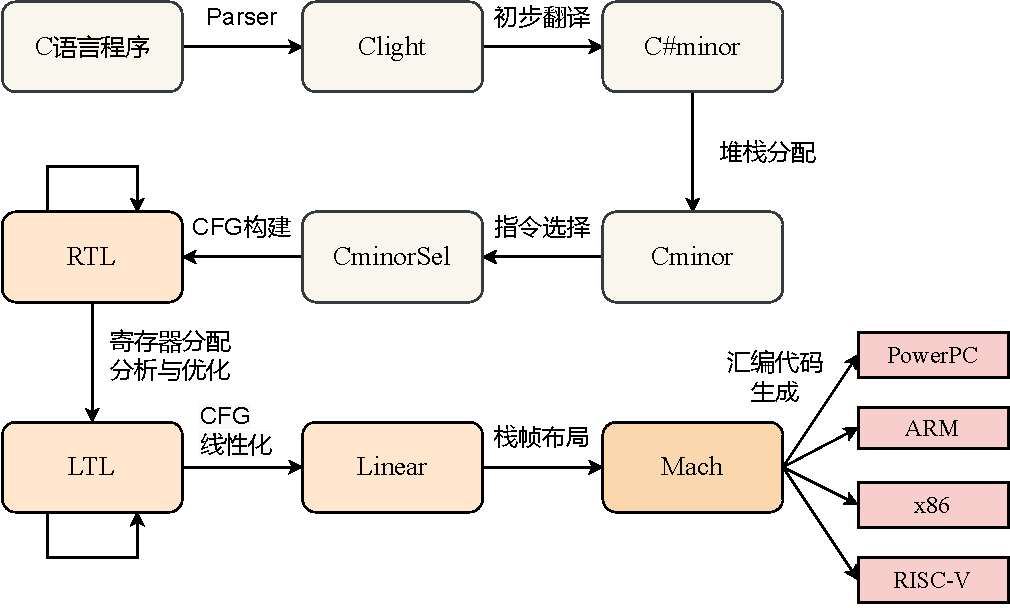
\includegraphics[width=0.8\linewidth]{figures/compcert.pdf}
    \caption{CompCert编译链概览}\label{fig:compcert}
\end{figure}

CompCertSSA是CompCert的一个扩展,具有一个基于SSA的中间端~\cite{compcertssa}。
它将SSA作为一种可选的优化中间语言,允许在RTL(Register Transfer Language)三地址代码和SSA中间语言之间进行转换。
CompCertSSA将RTL语言转换为SSA,经过全局值编号(Global Value Numbering,GVN)优化,再转换回RTL。
GVN优化是指对相同值的变量赋予相同的编号,从而消除冗余的计算。这里的SSA程序状态与RTL程序状态类似,
但是寄存器和当前函数类型要进行修改。在CompCertSSA中,$\phi$函数没有放在基本代码块中,
$\phi$指令代码块与普通指令构成的基本块是平行的结构。它们的语义也是平行定义的,
对基本代码块的控制流图定义了小步操作语义,对$\phi$指令代码块定义了大步操作语义。

虽然这使得CompCert能够实现一些基于SSA的优化~\cite{compcertssa-op,blazy-cpp2023},
但是CompCertSSA提供的优化仍然比较有限,不能与LLVM的后端优化相媲美。
本文中的SSA目标语言选择了接近LLVM中间语言的形式,也是为了对经验证的函数式语言编译器复用LLVM后端优化提供基础。
不过,它提供了一个从C语言开始的经过完整验证的编译链,是开发针对SSA的经验证的函数式编译器的有力工具。


\section{经验证的函数式编译器} \label{sec:relatedf}

许多经验证的函数式编译器选择与CompCert相连接~\cite{belanger2019certified, dargaye2009verification}。
经验证的函数式编译器CertiCoq将Gallina(Coq语言)编译到了CompCert中使用的的Clight~\cite{belanger2019certified}。
miniML经验证的编译器也使用了CompCert框架,将其编译到了CompCert中的中间语言Cminor~\cite{dargaye2009verification}。
也有经验证的函数式编译器选择了独立完成到汇编语言的编译链,例如CakeML~\cite{cakeml2016}。

\begin{itemize}
    \item \textbf{Gallina经验证的编译器CertiCoq:} 
    CertiCoq将Gallina编译到了C语言的子集Clight,以便与CompCert链接起来并最终编译到汇编语言,
    从而获得一个完整的经过验证的编译链~\cite{belanger2019certified,zoe-oopsla2021,zoe-icfp2021}。
    在CertiCoq中,源程序被转换为CPS形式后,经历了反柯里化(Uncurrying)、$\lambda$提升($\lambda$ Lifting)
    等优化~\cite{li2018verifying},并进行了闭包转换(Closure Conversion)~\cite{paraskevopoulou2019closure},
    确保函数没有包含非全局作用域的自由变量。之后,经过前述处理后得到的CPS程序就被转换到了Clight。
    尽管CertiCoq中使用的CPS语言,即L6语言,是一种纯函数式的语言,但是经过了前述的转换过程,
    研究者们能够较为直接地找出它与Clignt的对应关系。
    L6程序中的一个函数就对应着Clight中的一个函数。L6中所有的调用都是尾调用(Tail Call),并且C语言
    编译器CompCert实现了尾调用优化,可以将尾调用转换为跳转,不用创建新的栈帧。
    由于C语言没有自动的垃圾收集器(Garbage Collection),CertiCoq构造了与经验证的收集器的接口,
    并验证了该接口的正确性~\cite{wang2019certifying}。

    从CPS到Clight的编译过程及其形式化证明在Coq中实现,不过其使用的是大步操作语义而不是小步操作语义。
    其转换算法的正确性也使用了基于模拟的方法进行证明,证明了L6到Clight程序的前向模拟性质。
    该编译器的目标语言不是基于SSA的,因此不能直接连接到LLVM框架,也不能利用基于SSA中间语言的优化。
    \item \textbf{miniML经验证的编译器前端MLCompCert:} 
    MLCompCert是Zaynah Dargaye等人设计的一个经验证的编译器前端~\cite{dargaye2009verification}。
    它的源语言是ML纯函数式语言的部分,即miniML,包括了$\lambda$演算、$let$绑定、模式匹配等。
    它的目标语言是CompCert编译器后端的中间语言Cminor,即一种类似于C语言的底层语言。
    该编译器实现了一些经典的函数式程序编译优化,例如反柯里化和统一数据结构表示等。
    设计者们在Coq中对该函数式程序编译器前端进行了实现和验证。
    \item \textbf{经验证的函数式语言编译器CakeML:} 
    该编译器使用的源程序CakeML语言贴近实际中使用的函数式编程语言~\cite{cakeml2016}。
    它支持用户定义的模块、相互递归函数和模式匹配(Pattern Matching)等语言特性。
    CakeML编译器支持高效的柯里化多参数函数、可配置的数据表示、展开调用栈的异常、寄存器分配等功能。
    经过十几种中间语言的编译及优化过程,它最终将函数式语言编译到了机器码,支持32位及64位的ARM、RISC-V等不同架构。
    CakeML编译器为了提升寄存器分配的性能,会在进行寄存器分配之前对程序使用一个类似SSA化的转换,
    减小变量的生存期。由此转换步骤产生的程序并不严格符合SSA形式,它没有$\phi$函数。
    它使用隐式的$\phi$函数消除,用变量的移动替换$\phi$函数。
    该编译器的开发过程在HOL4定理证明工具中完成。
\end{itemize}


\section{基于SSA中间语言的编译器} \label{sec:relatedssa}

基于SSA的中间语言(例如LLVM IR)模块化、可移植和优化潜能大等特性引起了函数式编译器开发者的关注。
近年来,一些原本不使用SSA后端的函数式编译器已经开始转向SSA后端以获得更好的性能~\cite{farvardin2020new}。
在经验证的编译器领域,研究者们为了使用LLVM编译框架的优势,开始为LLVM IR提供形式化语义~\cite{zhao2012formalizing}。

\begin{itemize}
    \item \textbf{LLVM编译器框架:} 
    作为当今被广泛使用的主流编译器基础设施,LLVM(Low-Level Virtual Machine)编译器框架
    使用与程序执行平台无关的中间语言~\cite{lattner2004llvm}。这种中间语言是静态单赋值的,即每个变量只被赋值一次。
    基于LLVM框架的编译器在编译速度和目标程序的性能方面都有出色的表现,因此被广泛应用于学术界和工业界。
    如图~\ref{fig:llvm}所示,基于LLVM的编译器需要将源程序编译到LLVM IR。LLVM会提供针对LLVM IR程序的静态分析与优化工具,
    并能够将处理后的LLVM IR程序编译到不同目标架构的机器代码(包括x86、ARM等)。
    除了C和C++语言的编译器Clang的前端~\cite{lattner2008llvm},还有很多其他程序语言的编译器也使用LLVM框架。
    例如Haskell、Swift、Rust等语言也使用了将程序编译到LLVM中间语言的编译器,从而复用其后端~\cite{liu2013intel,zhang2012swift}。
    \begin{figure}[htbp]
        \centering
        \vspace{2ex}
        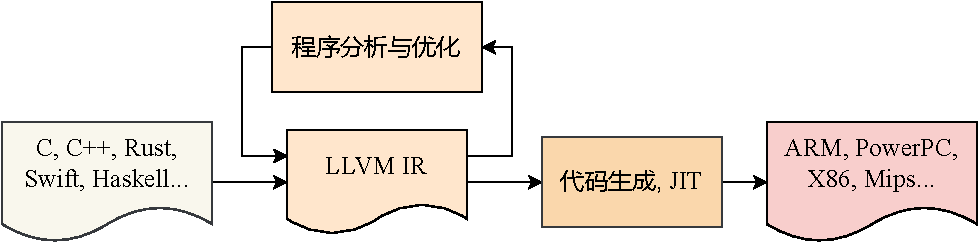
\includegraphics[width=0.8\linewidth]{figures/llvmst.pdf}
        \caption{LLVM编译框架}\label{fig:llvm}
    \end{figure}
    \item \textbf{SML-New Jersey基于LLVM编译器后端的版本:} 
    SML-New Jersey(SML/NJ)是一种经典的函数式编程语言。为了支持涌现出的各种不同的机器架构,
    SML/NJ的维护者们开发了MLRisc来作为抽象的机器层~\cite{george1994portable}。
    然而,在SML/NJ新发布的版本中,它更改了后端,将CPS中间语言编译到了LLVM IR~\cite{farvardin2020new}。
    这样的变更主要出于两种需求:为了利用LLVM编译器后端提供的丰富的分析与优化工具,以及为了支持更多的操作系统和机器架构。
    在新的SML/NJ编译器中,后端先读入高阶的CPS中间语言程序,将其转换为一阶程序,
    然后转换为控制流图(Control-Flow Graph, CFG)中间语言,再进一步转换为LLVM IR。
    使用LLVM框架之后的SML/NJ编译器生成的代码在性能上有所提升。
    但是,这项工作不是经过形式化验证的,无法保证高可靠性。
    我们的工作受到了这一趋势的启发,并进一步尝试对这种从CPS到SSA的连接进行形式化验证。
    \item \textbf{经验证的LLVM IR: Vellvm:} 
    Vellvm在定理证明工具Coq中定义了LLVM中间语言的抽象语法树(Abstract Syntax Tree, AST),并为LLVM IR提供了形式化语义。
    Vellvm还为其提供了类型系统及SSA结构相关性质的证明。
    研究者们还在Coq中实现了能够执行LLVM程序的解释器(Interpreter),来验证Vellvm的语义设计。
    利用Vellvm,我们可以将LLVM IR程序和它的Coq代码表示进行相互转换,还可以对针对LLVM IR的转换过程进行验证
    并直接插入到LLVM编译框架中。
    早期版本的Vellvm提供了LLVM IR的操作语义~\cite{zhao2012formalizing},
    而在较新版本中已迁移到了基于交互树(Interactive Tree, ITree)的语义~\cite{zakowski2021modular}。
    在本文第\ref{sec:overview}节所介绍的编译链中,SSA程序首先被编译到了Vellvm AST,然后生成了最终的LLVM IR程序。
\end{itemize}

\section{编译链概览} \label{sec:overview}

我们构建了一个从函数式语言PCF到LLVM IR的部分经过验证的编译器,并在Coq定理证明工具中
完成了编译算法和形式化验证的实现~\cite{chlipala2022certified}。
在本节中,我们主要是从高层次的角度介绍了这个编译器原型,省略了转换算法设计和证明定理的详细信息。
CPS转换及CPS到SSA转换的正确性通过源程序和目标程序之间的模拟进行形式化验证,
遵循第\ref{sec:compcertbackend}节中所介绍的CompCert后端的验证框架。
我们使用$\approx $表示语义保存性质。PCF、CPS和SSA的程序分别表示为$t_{pcf}$、$t_{cps}$和$t_{ssa}$。
通过对$t_{pcf}\approx t_{cps}$和$t_{cps}\approx t_{ssa}$的形式化证明,可以组合推导出$t_{pcf}\approx t_{ssa}$。
然后我们就得到了一个从PCF到SSA的经验证的编译过程。我们应用该经验证的编译过程,构建出一个编译器原型。
该编译器读取PCF程序,并经过图\ref{overview}中所示的几个编译步骤生成LLVM IR程序。

\begin{figure}[htbp]
    \centering
    \vspace{2ex}
    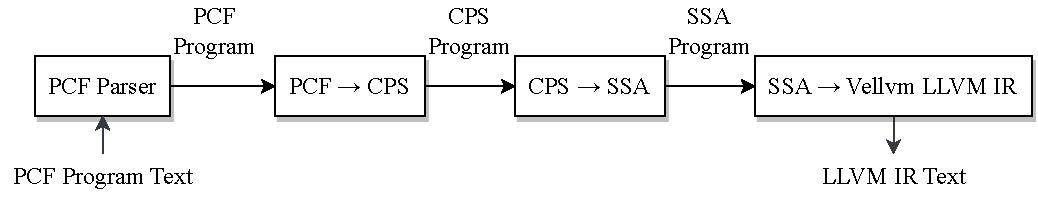
\includegraphics[width=0.8\linewidth]{figures/overview.pdf}
    \caption{PCF到LLVM编译链概览}\label{overview}
\end{figure}

\subsection{读入PCF文本}

使用PCF语法分析器(Parser)将文本形式的PCF程序提取为Coq中的结构化PCF代码项。
为了分析文本信息并提取PCF程序,获取源程序的语法结构至关重要。对于文本形式的PCF程序,
我们首先用词法分析器(Lexical Parser)将其解析为令牌(Token)流。
随后,使用语法分析器(Syntax Parser)分析该令牌流,生成Coq中的直接风格PCF程序项的抽象语法树。

\subsection{CPS转换}

如第\ref{sec:background}节中所言,函数式编程语言的编译器通常会将直接风格的程序转换为CPS形式,以获得显式的控制流。
我们已经得到了PCF程序的抽象语法树,但它是直接风格的程序,所以接下来需要使用CPS转换将其编译为CPS风格的程序。
将直接风格的PCF程序转换为CPS形式的算法主要由当前代码项和当前项被规约为某个值后要处理的下一个项决定。
另外,我们为直接风格及CPS风格的PCF语言定义了小步操作语义,并证明了CPS转换的前向模拟性质。
关于该CPS转换算法及其正确性验证的详细信息将在第\ref{sec:cpstrans}节和第\ref{sec:cpsforward}节中进行讨论。

\subsection{从CPS到SSA}

该编译链中最关键的部分是从CPS风格的函数式程序到目标SSA程序的转换及验证。
目标SSA语言是LLVM IR的简化版本,保留了其最基本的结构和程序语句。
通过该编译过程,输入的CPS程序项将被转换为一个包含主函数的SSA程序。
同样的,我们为这种SSA语言定义了小步操作语义,并证明了从CPS到SSA转换的前向模拟。
完成这一步证明后,我们将正向模拟组合起来,并完成了从源程序到SSA程序后向模拟的证明。
在第\ref{sec:cpsssatrans}节中将详细介绍该转换算法的设计和细节。
第\ref{sec:cpsssaforward}节中将进行CPS到SSA转换算法的形式化验证,并通过运行一个示例程序展示前向模拟的每一个关键步骤。

\subsection{从SSA到LLVM IR}

上一步中得到的SSA程序被转换为Vellvm中的抽象语法树,然后转换为LLVM IR程序文本。
在该编译链中,我们使用了经过验证的LLVM基础设施Vellvm~\cite{zakowski2021modular}。
利用其在Coq实现的LLVM IR的抽象语法树,我们可以进一步输出最终的LLVM IR程序。
由于我们使用的SSA语言是LLVM IR的简化版本,它保留了LLVM IR程序的基本结构,
可以方便地编译到Vellvm中的抽象语法树。这种SSA语言省略了LLVM IR中的大部分参数。
例如,函数定义在LLVM中非常复杂,有很多可选的参数,而本文中的SSA语言只保留了函数定义中必须指定的内容。
LLVM中的表达式类型多种多样,其中整数包括多种宽度的i16、i32等,
而本文的SSA语言简化为没有明确指定类型的无限宽自然数。
该编译过程的主要工作其实就是为这些被省略的参数选取正确的默认值。

% !TEX root = ../main.tex

\chapter{CPS到SSA中间语言的转换算法} \label{ch:trans}

\section{源语言:CPS形式的PCF语言} \label{sec:cps}

PCF(Programming Computable Functions)是一种被广泛应用于研究的函数式语言~\cite{plotkin1977lcf}。
尽管PCF是一种小规模的语言,但它是图灵完备的,即所有可计算的函数都可以表示为PCF程序。
把它作为该编译框架的源语言,不会使算法和验证过于复杂而无法完成,也能够说明关键问题。
在本节中,我们定义了直接风格和CPS形式PCF语言的语法和小步操作语义。
我们还展示了将直接风格PCF转换为CPS形式的算法。

\subsection{源语言的语法和语义}

本文中介绍的PCF语言来自Dowek和L{'e}vy的工作~\cite{dowek2010introduction}。
它包括基本的$\lambda$-演算、算术运算表达式、条件表达式和不动点(Fixed Point)。PCF及其CPS形式的语法定义如图~\ref{pcfsyntax}所示。

\begin{figure}[htbp]
        \centering
        \begin{subfigure}[b]{0.4\textwidth}
            \flushright
        \begin{equation}
            \nonumber
            \begin{aligned}
                op\, := &\; +\; |\; -\; | \; \times \; |\; \div \\
                t\, := &\; i\; |\; x\; |\; t_1\; t_2\; |\; \mathbf{ifz}\; t_1\; t_2\; t_3 \\
                & |\; op\; t_1\; t_2 \\
                & |\; \mathbf{let}\; x=t_1\; \mathbf{in}\; t_2 \\
                & |\; \mathbf{fix}\; f\; x\; t
            \end{aligned}
        \end{equation}
        \caption{直接风格的PCF语言语法}\label{directpcf}
        \end{subfigure}
       % \hfill
        \begin{subfigure}[b]{0.5\textwidth}
            \flushleft
        \begin{equation}
            \nonumber
            \begin{aligned}
                v\, := &\; i\; |\; x \\
                t\, := &\; \mathbf{letval}\; x=v\; \mathbf{in}\; t\; |\; k\; v\; |\; \mathbf{ifz}\; v\; t_1\; t_2 \\
                & |\; f\; k\; v\; |\; \mathbf{letop}\; x=op\; x_1\; x_2\; \mathbf{in}\; t \\
                & |\; \mathbf{letcont}\; k\; x=t_1\; \mathbf{in}\; t_2 \\
                & |\; \mathbf{letfun}\; f\; k\; x=t_1\; \mathbf{in}\; t_2 
            \end{aligned}
        \end{equation}
        \caption{CPS形式的PCF语言语法}\label{cpspcf}
    \end{subfigure}
    \caption{PCF语言语法}\label{pcfsyntax}
    \end{figure}

最基本的PCF代码项(Term)包含自然数$i$和变量$x$。将代码项$t_1$应用到代码项$t_2$上表示为$t_1\; t_2$。
我们使用$\mathbf{let}\; x = t_1\; \mathbf{in}\; t_2$表示在$t_2$中将变量$x$替换为$t_1$的值。
PCF中的条件表达式记作$\mathbf{ifz}\; t_1\; t_2\; t_3$。如果$t_1$的值为0,则整个代码项规约到$t_2$。
否则,它将规约到$t_3$。PCF中的不动点代码项是$\mathbf{fix}\; f\; x\; t$,其中$t$中可能出现$f$。
例如,图~\ref{factpcf}中展示了使用直接风格的PCF实现阶乘功能并应用到参数2的程序。

CPS形式的PCF语言遵循Kennedy提出的CPS风格函数式程序结构~\cite{kennedy2007compiling}。
值$v$在CPS项中可以通过$\mathbf{letval}\; x = v\; \mathbf{in}\; t$语句引入。$k\; v$将延续(Continuation)$k$应用于参数$v$。
$f\; k\; v$将函数$f$应用于参数$v$,并传递延续变量$k$以接受此调用返回的结果。
语句$\mathbf{letop}\; x = op\; x_1\; x_2\; \mathbf{in}\; t$将变量$x$在项$t$中绑定为该二元运算的结果。
通过$\mathbf{letcont}\; k\; x = t_1\; \mathbf{in}\; t_2$引入局部延续(Local Continuation)$k$,其中$t_1$是延续$k$的延续体(Body)。
$\mathbf{letfun}\; f\; k\; x = t_1\; \mathbf{in}\; t_2$构造一个返回延续(Return Continuation)为$k$的函数$f$。
图~\ref{factcps}描述了CPS形式的PCF语言中阶乘函数的实现及对参数2的应用,其中每个计算步骤都是被显式命名的。
可以看到,顶层延续变量$k_{init}$接受整个程序返回的结果,并由其上下文绑定。

\begin{figure}[htbp]
        \centering
        \begin{subfigure}[b]{0.3\textwidth}
            \flushright
        % \small
        \begin{equation}
            \nonumber
            \begin{aligned}
            & (\mathbf{fix}\; fact\; x \\
            & \quad \mathbf{ifz}\; x\; 1 \\
            & \quad\quad (x*(fact\; (x-1)))) \\
            & 2
            \end{aligned}
        \end{equation}
        \caption{直接风格的PCF阶乘程序}\label{factpcf}
        \end{subfigure}
        \begin{subfigure}[b]{0.68\textwidth}
            \flushleft
            % \small
        \begin{equation}
            \nonumber
            \begin{aligned}
            & \mathbf{letfun}\; fact\; k\; x = (\mathbf{ifz}\; x\; (\mathbf{letval}\; x_1=1\; \mathbf{in}\; (k\; x_1))\\
            & \quad (\mathbf{letval}\; x_2=1\; \mathbf{in}\; (\mathbf{letop}\; x_4=x-x_2\; \mathbf{in} \\
            & \quad\quad \mathbf{letcont}\; k_1\; z= (\mathbf{letop}\; x_3=x*z\; \mathbf{in}\; (k\; x_3))\\
            & \quad\quad\quad  \mathbf{in}\; fact\; k_1\; x_4)))\; \mathbf{in} \\
            & (\mathbf{letval}\; x_5=2\; \mathbf{in}\; (\mathbf{letcont}\; k_2\; y=k_{init}\; y\; \mathbf{in}\; (fact\; k_2\; x_5))) \\
            \end{aligned}
        \end{equation}
        \caption{CPS形式的PCF阶乘程序}\label{factcps}
        \end{subfigure}
    \caption{使用PCF语言实现阶乘程序}\label{factpcfcps}
    \end{figure}

接下来,我们需要为以上所介绍的PCF语言提供小步操作语义。
$S\rightarrow S'$表示执行一步操作可以使程序从初始状态$S$到达状态$S'$。
在直接风格的PCF程序中,程序状态之间的转换步骤表示为:
\begin{equation}
(t_{pcf},ctx)\rightarrow (t'_{pcf},ctx').
\end{equation}
$t_{pcf}$表示的是正在被求值(Evaluate)的表达式的PCF代码项。
$ctx$是一个包含代码项序列的上下文(Context),用于在当前$t_{pcf}$的求值完成后进行下一步执行操作。
当$ctx = ctx_{stop}$时,程序执行在$t_{pcf}$求值完成后即可结束。否则,当$ctx = ctx_{seq}\; t\; ctx$,
表示$t_{pcf}$的值将作为后续代码项$t$的参数,程序继续执行。经过一步转换之后,
新的程序状态包含了更新后的PCF代码项$t'_{pcf}$和新的上下文$ctx'$。转换规则如图~\ref{pcfopsem}所示。

$\mathbf{let}$表达式在$t_2$中用代码项$t_1$的值替换变量$x$。
因此,我们首先对$t_1$进行求值并将当前求值完成后下一步需要处理的代码项追加在上下文$ctx$中。
然后,在得到$t_1$的值后,我们将$t_2$中的变量$x$进行替换。当将不动点应用于代码项$t_2$时,
也是进行类似的操作。先将不动点放入上下文中,当$t_2$的值计算完毕后,将用它来替换不动点中的参数$x$,然后计算继续进行。
对于$\mathbf{ifz}$条件语句,我们求出$t_1$的值$n$,并根据$n$是否为0来确定下一步规约操作。

\begin{figure}[t]
    \centering
    \begin{subfigure}[t]{0.43\textwidth}
        \setlength{\jot}{10pt}
        \begin{gather*}
            \displaystyle{\frac{t_{pcf}=(\mathbf{let}\; x = t_1\; \mathbf{in}\; t_2)} {(t_{pcf},\; ctx)\rightarrow (t_1,\; ctx_{seq}\; t_{pcf}\; ctx)}} \\
            \displaystyle{\frac{t_1\; is\; a\; value\quad t_3=(\mathbf{let}\; x = t_1\; \mathbf{in}\; t_2)} {(t_1,\; ctx_{seq}\; t_3\; ctx)\rightarrow (t_2 [t_1/x],\; ctx)}} \\
            \displaystyle{\frac{v\; is\; a\; value\quad t_3=(\mathbf{ifz}\; t_1\; t_2\; t_3)} {(v,\; ctx_{seq}\; t_3\; ctx)\rightarrow (t_3 [v/t_1],\; ctx)}} \\
            \displaystyle{\frac{t_{pcf}=(\mathbf{ifz}\; t_1\; t_2\; t_3)} {(t_{pcf},\; ctx)\rightarrow (t_1,\; ctx_{seq}\; t_{pcf}\; ctx)}} \\
            \displaystyle{(\mathbf{ifz}\; 0\; t_2\; t_3,\; ctx)\rightarrow (t_2,\; ctx)} \\
            \displaystyle{\frac{n \neq 0}{(\mathbf{ifz}\; n\; t_2\; t_3,\; ctx)\rightarrow (t_3,\; ctx)}} \\
        \end{gather*}
    \end{subfigure}
    \begin{subfigure}[t]{0.55\textwidth}
        \setlength{\jot}{10pt}
        \begin{gather*}
            \displaystyle{\frac{t_{pcf}=((\mathbf{fix}\; f\; x\; t_1)\; t_2)} {(t_{pcf},\; ctx)\rightarrow (t_2,\; ctx_{seq}\; (\mathbf{fix}\; f\; x\; t_1)\; ctx)}} \\
            \displaystyle{\frac{t_2\; is\; a\; value\quad t_3=(\mathbf{fix}\; f\; x\; t_1)} {(t_2,\; ctx_{seq}\; t_3\; ctx)\rightarrow (t_1 [t_2/x,t_3/f],\; ctx)}} \\
            \displaystyle{(op\; t_1\; t_2,\; ctx)\rightarrow (t_1,\; ctx_{seq}\; (op\; t_1\; t_2,\; ctx)\; ctx)} \\
            \displaystyle{\frac{v_1\; is\; a\; value\quad t_3=(op\; t_1\; t_2,\; ctx)} {(v_1,\; ctx_{seq}\; t_3\; ctx)\rightarrow (t_2,\; ctx_{seq}\; (op\; v_1\; t_2)\; ctx)}} \\
            \displaystyle{\frac{v_1,\; v_2\; are\; values\quad n=\mathbf{eval}_{op}\; op\; v_1\; v_2}{(v_2,\; ctx_{seq}\; (op\; v_1\; t_2)\; ctx)\rightarrow (n,\; ctx)}} \\
        \end{gather*}
    \end{subfigure}   
    \caption{直接风格的PCF语言小步操作语义转换规则} \label{pcfopsem}
\end{figure}

CPS形式的PCF语言的小步操作语义表示的推导规则形如
\begin{equation}
(t_{cps},loc_{cps})\rightarrow(t'_{cps},loc'_{cps}).
\end{equation}
同样的,$t_{cps}$是正在被计算的CPS代码项,$loc_{cps}$是从延续变量名或函数名到引入它们的代码项的映射(Mapping)。
$t'_{cps}$和$loc'_{cps}$分别是更新后的CPS代码项和映射。
CPS形式的PCF语言的小步操作语义转换规则如图~\ref{cpsopsem}所示。
$\mathbf{letval}$表达式可以将新的值引入代码项$t$,我们只需要在$t$中用$v$替换变量$x$。
对于代码项$(\mathbf{letcont}\; k\; x=t_1\; \mathbf{in}\; t_2)$,
首先对$t_2$求值并更新$loc_{cps}$,添加从延续变量$k$到该代码项的映射。
我们使用$loc_{cps}\; [k\mapsto t_{cps}]$这种标记来表示对映射$loc_{cps}$的更新操作。
当把延续$k$应用于值$v$时(用$k\; v$表示),由于$t_1$是延续$k$的延续体,我们将$t_1$中的变量$x$替换为$v$。
$\mathbf{letfun}$代码项的规约与之类似,当我们遇到$\mathbf{letfun}$结构时,我们会更新从$f$到该项的映射。
当我们将延续$k_0$和变量$x_0$作为参数传递给$f$时,我们分别用$k_0$和$x_0$替换函数体$t_1$中的$k$和$x$。

\begin{figure}[htbp]
    \centering
    \begin{subfigure}[t]{0.43\textwidth}
        \setlength{\jot}{10pt}
        \begin{gather*}
            \displaystyle{\frac{t_{cps}=(\mathbf{letval}\; x=v\; \mathbf{in}\; t)} {(t_{cps},\; loc_{cps})\rightarrow (t [v/x],\; loc_{cps})}} \\
            \displaystyle{\frac{t_{cps}=(\mathbf{ifz}\; 0\; t_1\; t_2)} {(t_{cps},\; loc_{cps})\rightarrow (t_1,\; loc_{cps})}} \\
            \displaystyle{\frac{t_{cps}=(\mathbf{ifz}\; n\; t_1\; t_2)\quad n \neq 0} {(t_{cps},\; loc_{cps})\rightarrow (t_2,\; loc_{cps})}} \\
            \displaystyle{\frac{loc_{cps}\; k = (\mathbf{letcont}\; k\; x=t_1\; \mathbf{in}\; t_2)}{(k\; v,\; loc_{cps})\rightarrow (t_1 [v/x],\; loc_{cps})}} \\
        \end{gather*}
    \end{subfigure}
    \begin{subfigure}[t]{0.55\textwidth}
        \setlength{\jot}{10pt}
        \begin{gather*}
            \displaystyle{\frac{t_{cps}=(\mathbf{letop}\; x=op\; v_1\; v_2\; \mathbf{in}\; t)}
            {(t_{cps},\; loc_{cps})\rightarrow (t [(\mathbf{eval}_{op}\; op\; v_1\; v_2)/x],\; loc_{cps})}} \\
            \displaystyle{\frac{t_{cps}=(\mathbf{letfun}\; f\; k\; x=t_1\; \mathbf{in}\; t_2)} {(t_{cps},\; loc_{cps})\rightarrow (t_2,\; loc_{cps}\; [f\mapsto t_{cps}])}} \\
            \quad \displaystyle{\frac{loc_{cps}\; f = (\mathbf{letfun}\; f\; k\; x=t_1\; \mathbf{in}\; t_2)}{(f\; k_0\; x_0,\; loc_{cps})\rightarrow (t_1 [x_0/x, k_0/k],\; loc_{cps})}} \\
            \displaystyle{\frac{t_{cps}=(\mathbf{letcont}\; k\; x=t_1\; \mathbf{in}\; t_2)} {(t_{cps},\; loc_{cps})\rightarrow (t_2,\; loc_{cps}\; [k\mapsto t_{cps}])}} 
        \end{gather*}
    \end{subfigure}   
    \caption{CPS形式的PCF语言小步操作语义转换规则}\label{cpsopsem}
\end{figure}

\subsection{直接风格PCF语言的CPS转换} \label{sec:cpstrans}

如第\ref{sec:bg_cps}节中所述,函数式语言的编译器通常会将直接风格的源程序转换为CPS形式,
即进行CPS转换(CPS Transformation)。本节中,我们将介绍把PCF源程序转换为CPS形式的编译算法。
该算法遵循CPS转换的一般模式~\cite{plotkin1975call,danvy2007one},根据计算的层次顺序递归地解构处理PCF代码项。
例如,如果PCF代码项$t$的计算步骤可以有序地分为对$t_1$和$t_2$的计算,
那么我们就可以把对$t_2$进行转换得到的CPS代码项放入之后要处理的参数中,并在下一步中直接开始处理$t_1$。 

转换过程由图~\ref{algo:cpstrans}中的函数$\mathcal{F}_{proc}$描述,它使用了一个更加广义的转换函数$\mathcal{F}$。
函数$\mathcal{F}$的输入和输出分别表示为$(t_{pcf}, l_v, \kappa)$和$t_{cps}$。
$t_{pcf}$是待转换的PCF程序。$\kappa$的结构表示为$\lambda x. t'_{cps}$,
代表了当前代码项被归约到一个值后要被应用的CPS代码项(延续)。$t_{cps}$是其生成的CPS程序。
在我们的CPS转换算法中,变量使用有名字的字符串名称。$l_v$是已经被使用的变量列表,
新生成的名称不能与$l_v$中的名称冲突。例如,使用图~\ref{algo:cpstrans}中的规则(3)对$t_1\; t_2$进行转换,
生成的新变量$k,\, x,\, y,\, z$必须不能已经存在于$l_v$中。该步转换之后,它们被添加到$l_v$中。
为了简化转换规则,我们没有在图中的算法里写出使用$l_v$指定生成新变量的具体操作。
它所做的其实是通过维护最新生成的变量的下标,来选择最小未使用的正数作为新变量的下标。
在初始状态中,要转换的PCF程序即为源程序$t_{pcf}$,新生成的名称只有顶层延续变量的名字$k_{init}$。
此时参数$\kappa$为$\lambda x. (k_{init}\; x)$,表示它接受整个生成的$t_{cps}$程序的值。
因此,应用$k_{init}$的值将是程序的最终结果。

\begin{figure}[t]
    \centering
    % \small
    % \setlength{\jot}{10pt}
    \begin{algorithm}[H]
        \caption{CPS转换}
        \SetAlgoLined
        $\mathcal{F}_{proc}:\quad \mathbf{Input:}\; t_{pcf}\quad \mathbf{Output:}\; t_{cps}$\\
        $\mathcal{F}_{proc}(t_{pcf})\coloneqq \mathbf{\mathcal{F}}(t_{pcf}, [k_{init}], \lambda x. (k_{init}\; x))$\\
        \vspace*{0.5em}
        $\mathcal{F}:\quad \mathbf{Input:}\; t_{pcf},\; l_v,\; \kappa \quad \mathbf{Output:}\; t_{cps}$\\ 
        $(1).\; \mathbf{\mathcal{F}}(i, l_v, \kappa) \coloneqq \textcolor{blue}{\mathbf{letval}\; x= i\; \mathbf{in}\; \kappa(x)} $ \\
        $(2).\; \mathbf{\mathcal{F}}(x, l_v, \kappa) \coloneqq \kappa(x) $ \\
        $(3).\; \mathbf{\mathcal{F}}(t_1\; t_2, l_v, \kappa) \coloneqq \mathbf{\mathcal{F}}(t_1, l'_v,\lambda x. \mathbf{\mathcal{F}}(t_2, l'_v, \lambda y. (\textcolor{blue}{\mathbf{letcont}\; k\; z=\kappa(z)\; \mathbf{in}\; (x\; k\; y)})))$ \\
        $\quad\quad \mathtt{where}\; l'_v = l_v \doubleplus [k;x;y;z]$ \\
        $(4).\; \mathbf{\mathcal{F}}(\mathbf{ifz}\; t_1\; t_2\; t_3, l_v, \kappa) \coloneqq \mathbf{\mathcal{F}}(t_1, l'_v, \lambda x. (\textcolor{blue}{\mathbf{ifz}\; x\; \mathbf{\mathcal{F}}(t_2, l'_v, \kappa)\; \mathbf{\mathcal{F}}(t_3, l'_v, \kappa)}))  $ \\
        $\quad\quad \mathtt{where}\; l'_v = l_v \doubleplus [x]$ \\
        $(5).\; \mathbf{\mathcal{F}}(op\; t_1\; t_2, l_v, \kappa) \coloneqq \mathbf{\mathcal{F}}(t_1, l'_v,\lambda x.\mathbf{\mathcal{F}}(t_2, l'_v, \lambda y. (\textcolor{blue}{\mathbf{letop}\; z=op\; x\; y\; \mathbf{in}\; \kappa(z)}))) $ \\
        $\quad\quad \mathtt{where}\; l'_v = l_v \doubleplus [x;y;z]$ \\
        $(6).\; \mathbf{\mathcal{F}}(\mathbf{let}\; x=t_1\; \mathbf{in}\; t_2, l_v, \kappa) \coloneqq \mathbf{\mathcal{F}}(t_1, l_v, \lambda x. \mathbf{\mathcal{F}}(t_2, l_v, \kappa)) $ \\
        $(7).\; \mathbf{\mathcal{F}}(\mathbf{fix}\; f\; x\; t, l_v, \kappa) \coloneqq \textcolor{blue}{\mathbf{letfun}\; f\; k\; x= \mathbf{\mathcal{F}}(t, l'_v, \lambda y. (k\; y))\; \mathbf{in}\; \kappa(f)}$ \\
        $\quad\quad \mathtt{where}\; l'_v = l_v \doubleplus [k;y]$
    \end{algorithm}
    \caption{CPS转换算法}\label{algo:cpstrans}
\end{figure}

接下来,我们将以图~\ref{factpcfcps}中的直接风格与CPS形式PCF程序为例,说明以上CPS转换算法是如何将
图~\ref{factpcf}中的程序转换为图~\ref{factcps}中的程序。说明过程中我们会略去新变量名的生成方法
和$l_v$参数的维护,因为它们始终遵循同样的方法,不需再逐步描述。以下说明中已生成变量名参数均记为$l_v$。

\begin{enumerate}
    \item 首先对CPS源程序应用图~\ref{algo:cpstrans}中的规则(3),下一步需要处理的PCF程序变为
        子代码项$\mathbf{fix}\; fact\; x\; \dots$,参数$\kappa $从初始状态时的$\lambda x. (k_{init}\; x)$变为
        $\lambda x. \mathbf{\mathcal{F}}(2, l_v, \lambda z. $ \\ $(\mathbf{letcont}\; k_2\; y=k_{init}\; y\; \mathbf{in}\; (x\; k_2\; z)))$。
    \item 先对参数$\kappa $中的$\mathbf{\mathcal{F}}$进行处理。根据规则(1),我们添加$\mathbf{letval}$结构并用$x_5$替换绑定变量$z$,它转换为
        $\mathbf{letval}\; x_5 = 2\; \mathbf{in}\; (\mathbf{letcont}\; k_2\; y=k_{init}\; y\; \mathbf{in}\; (x\; k_2\; x_5))$。
        我们将其记为$t_{cps1}$,那么当前的参数$\kappa $就是$\lambda x. t_{cps1}$。
    \item 根据规则(7)处理$\mathbf{fix}$代码项,$\kappa(fact)$就是将$t_{cps1}$中的绑定变量名$x$替换为$fact$,
    把$\mathbf{fix}$代码项的函数体部分记为$t_{cps2}$,CPS转换的目标程序变为:
    \begin{equation}
        \nonumber
        \begin{aligned}
        & \mathbf{letfun}\; fact\; k\; x = \mathbf{\mathcal{F}}(t_{cps2}, l_v, \lambda y. (k\; y))\; \mathbf{in} \\
        & \quad (\mathbf{letval}\; x_5=2\; \mathbf{in}\; (\mathbf{letcont}\; k_2\; y=k_{init}\; y\; \mathbf{in}\; (fact\; k_2\; x_5))) \\
        \end{aligned}
    \end{equation}
    \item 接下来的任务就是求出$\mathbf{\mathcal{F}}(t_{cps2}, l_v, \lambda y. (k\; y))$。
        由于$t_{cps2}$是一个条件表达式,我们使用规则(4)处理它。
        将当前的$\kappa$参数记为$\kappa_1$,将PCF子代码项$(x*(fact\; (x-1)))$记为$t_{cps3}$,目标转换为
        $\mathbf{\mathcal{F}}(x, l_v, \lambda y. (\mathbf{ifz}\; y\; \mathbf{\mathcal{F}}(1, l_v, \kappa_1)\; \mathbf{\mathcal{F}}(t_{cps3}, l_v, \kappa_1)))$。
        按照规则(2),待处理PCF为变量时可以直接把当前的参数$\kappa$应用到变量$x$上。对于$\mathbf{\mathcal{F}}(1, l_v, \kappa_1)$可以使用规则(1)。
        目标转换为$\mathbf{ifz}\; x\; \mathbf{letval}\; x_1 = 1\; \mathbf{in}\; (k\; x_1)\; \mathbf{\mathcal{F}}(t_{cps3}, $ \\ $l_v, \kappa_1)$。
    \item 问题转换为求出$\mathbf{\mathcal{F}}(t_{cps3}, l_v, \kappa_1)$。对于二元算术运算,我们按照规则(5)进行处理。
        由于第一个操作数$x$是一个变量,我们可以直接用它来替换新的参数$\kappa$中的绑定变量。
        待求的程序变为$\mathbf{\mathcal{F}}(fact\; (x-1), l_v, \lambda m. (\mathbf{letop}\; x_3=x*m\; \mathbf{in}\; k\; x_3))$。
        $fact$是函数名,同时也是变量名。将其应用到$(x-1)$上可以使用转换规则(3)。
    \item 由于规则(1)、(2)、(3)和(5)在前几步的转换中都已经使用过,之后的转换步骤还是运用这几条规则,在此不再详述。
        最终,我们得到的CPS目标程序就是图~\ref{factcps}所示的程序。
\end{enumerate}

\section{目标语言:类似LLVM IR的SSA语言}

本文中使用的目标SSA语言是一种简化版本的LLVM IR,保留了其最基本的程序结构层次。
在本节接下来的内容中,我们将定义它的语法和小步操作语义,并讨论对SSA程序中自由变量的处理和避免。

\subsection{目标语言的语法和语义}

\begin{figure}[htbp]
    \centering
    \begin{equation}
        \nonumber
        \begin{aligned}
            l &\coloneqq string & v &\coloneqq i\; |\; x & r &\coloneqq \mathbf{ret}\; v\; |\; \mathbf{br_{uc}}\; l\; |\; \mathbf{br_c}\; v\; l_1\; l_2 \\
            \phi_a &\coloneqq (l,\; v) & \phi &\coloneqq x = \overline{\phi_a} &  c &\coloneqq v\; |\; op\; v_1\; v_2\; |\; \mathbf{icmp}\; v_1\; v_2\; |\; \mathbf{call}\; x\; v \\
            a &\coloneqq x = c; & b &\coloneqq l:\; \overline{\phi}\; \overline{a}\; r & f &\coloneqq \mathbf{define}\; l_1(l_2)\; \overline{b} \quad\quad\quad t \coloneqq \overline{f} \\
        \end{aligned}
    \end{equation}
    \caption{SSA目标语言的语法}\label{synssa}
\end{figure}

我们使用的目标SSA语言的语法定义如图~\ref{synssa}所示。
顶层的翻译单元(Translation Unit)$t$由一系列函数定义组成。
一个函数$f$包含函数名$l_1$、参数$l_2$和一系列基本代码块$\overline{b}$。
一个基本代码块$b$由它的标签$l$、$\overline{\phi}$节点序列、指令$\overline{a}$序列和一个终止指令(Terminator)$r$组成。
一条指令$a$将命令$c$的值赋给变量$x$。$c$包括值$v$、二元运算表达式、比较两个值是否相等的命令和函数调用。
终止指令包括$\mathbf{ret}$和$\mathbf{br}$,分别用于表示函数返回和块之间的跳转。
作为示例程序,图~\ref{factssa}展示了SSA中的阶乘函数与2的阶乘。

\begin{figure}[ht]
    \centering
    \begin{equation}
        \nonumber
        \begin{aligned}
            & \mathbf{define}\; fact\; (x)\\
            & \quad b_1:\; b_0 = \mathbf{icmp}\; x\; 0;\; \mathbf{br_c}\; b_0\; t_0\; f_0; \\
            & \quad t_0:\; x_1 = 1;\; r_{t0} = x_1;\; \mathbf{ret}\; r_{t0}; \\
            & \quad f_0:\; x_2 = 1;\; x_4 = x - x_2;\; z = \mathbf{call}\; fact\; x_4;\; \mathbf{br_{uc}}\; k_1; \\
            & \quad k_1:\; x_3 = x*z;\; r_{k1} = x_3;\; \mathbf{ret}\; r_{k1}; \\
            & \mathbf{define}\; main\; ( )\\
            & \quad b_1:\; x_5 = 2;\; y = \mathbf{call}\; fact\; x_5;\; \mathbf{br_{uc}}\; k_2;\\
            & \quad k_2:\; r_{k2} = y;\; \mathbf{ret}\; r_{k2};
        \end{aligned}
    \end{equation}
    \caption{SSA语言中的阶乘程序}\label{factssa}
\end{figure}

目标SSA语言的小步操作语义规则表示为
\begin{equation}
(pc, ppc, loc_{ssa}, s_{ssa}) \rightarrow (pc', ppc', loc'_{ssa}, s'_{ssa}).
\end{equation}
$pc$是程序计数器(Program Counter),用于定位当前指令,由三个元素$(l_{f}, l_b, n)$组合而成。
其中,$l_{f}$是当前函数标签,$l_b$是当前基本代码块标签,$n$表示基本块中指令的位置。
可以使用$\mathbf{code}_{at}\; pc$获取$pc$位置处的指令。$ppc$存储了上一个块中进行跳转之前的程序计数器值,
以便对$\phi$-节点进行求值。$loc_{ssa}$是变量名到它们的值的映射。
我们在堆栈$s_{ssa}$中保留调用当前函数的指令的程序计数器,以便在当前函数返回时能够返回到调用时的位置。

SSA语言的操作语义转换规则如图~\ref{ssaopsem}所示。
第一条规则描述了函数调用的程序状态转换。
控制流跳转到函数$f$的开头,并将函数返回地址存储在$s_{ssa}$中。
$\mathbf{arg}\; f$表示获取函数$f$的参数,$loc_{ssa}\; [x\mapsto v_0]$表示把从$x$到$v_0$的映射添加到$loc_{ssa}$中。
例如,在图~\ref{factssa}中,当主函数调用$fact$函数时,按照图~\ref{ssaopsem}中的第一条规则,
程序状态从$((main,b_1,1),\, (main,empty,1),\, loc_{ssa},\, s_{ssa})$ 
转换到$((fact,b_1,0),\, (main,b_1,1),\, loc_{ssa}$ \\ $[x\mapsto 2],\, \mathbf{push}\; s_{ssa}\; (main,b_1,1))$。
第二条规则定义了当前函数返回并将返回值传递给调用语句时发生的状态转换。
它从$s_{ssa}$的顶部取出程序计数器$npc$,存储返回值,并跳回该调用语句的位置。
对于$\phi$-节点,我们利用$ppc$提供的信息得到前驱基本块的标签,从而确定变量$x$被赋予的值是哪个版本。
二元算术运算语句、普通赋值语句和$\mathbf{icmp}$语句的处理方法类似,都是利用$loc_{ssa}$计算变量被赋予的具体值,并更新到映射中。
在我们的SSA程序中,变量被使用之前一定是被赋值过的,所以可以计算出这些语句等号右边表达式结果值。
对于无条件跳转和条件跳转语句,由于它们只是同一函数内不同基本代码块之间的跳转,我们只需求出新的基本块标签。
当然,在下一个程序状态中$ppc$就变成了当前状态的$pc$。

\begin{figure}[htbp]
    % \vspace*{-0.3cm}
    \centering
    % \small
    \setlength{\jot}{10pt}
    \begin{gather*}
        \displaystyle{\frac{\mathbf{code}_{at}\; pc\; =\; (y=\mathbf{call}\; f\; v_0)\quad \mathbf{arg}\; f = x}
        {(pc,\; ppc,\; loc_{ssa},\; s_{ssa})\rightarrow ((f,b_1,0),\; pc,\; loc_{ssa}\; [x\mapsto v_0],\; \mathbf{push}\; s_{ssa}\; pc )}} \\
        % & \displaystyle{\frac{\mathbf{code}_{at}\; pc\; =\; id = phi,\quad n = \mathbf{eval}_{phi}\ phi\ ppc\ loc_{ssa} } {(pc,\; ppc,\; loc_{ssa},\; ploc_{ssa})\rightarrow (pc+1,\; ppc,\; loc_{ssa}\; id\mapsto n,\; ploc_{ssa})}} \\
        \displaystyle{\frac{\begin{matrix}\mathbf{code}_{at}\; pc\; =\; (\mathbf{ret}\; v)\quad pc.l_f \neq main\quad npc = \mathbf{top}\; s_{ssa}
        \\ \mathbf{code}_{at}\; npc\; =\; (x=\mathbf{call}\; f\; v_0)\end{matrix}} 
        {(pc,\; ppc,\; loc_{ssa},\; s_{ssa})\rightarrow (npc+1,\; pc,\; loc_{ssa}\; [x\mapsto v],\; \mathbf{pop}\; s_{ssa})}} \\
        \displaystyle{\frac{\mathbf{code}_{at}\; pc\; =\; (x=\overline{\phi_a})\quad n\; =\; \mathbf{eval}_{\phi}\ \overline{\phi_a}\ ppc}
            {(pc,\; ppc,\; loc_{ssa},\; s_{ssa})\rightarrow (pc+1,\; ppc,\; loc_{ssa}\; [x\mapsto n],\; s_{ssa})}} \\
        \displaystyle{\frac{\mathbf{code}_{at}\; pc\; =\; (x=op\; v_1\; v_2)\quad n\; =\; \mathbf{eval}_{exp}\ loc_{ssa}\ op\; v_1\; v_2}
        {(pc,\; ppc,\; loc_{ssa},\; s_{ssa})\rightarrow (pc+1,\; ppc,\; loc_{ssa}\; [x\mapsto n],\; s_{ssa})}} \\
        \displaystyle{\frac{\mathbf{code}_{at}\; pc\; =\; (x=v)\quad n\; =\; v\; is\; value?\; v\; :\; (loc_{ssa}\; v)}
        {(pc,\; ppc,\; loc_{ssa},\; s_{ssa})\rightarrow (pc+1,\; ppc,\; loc_{ssa}\; [x\mapsto n],\; s_{ssa})}} \\
        \displaystyle{\frac{\mathbf{code}_{at}\; pc\; =\; (x=\mathbf{icmp}\; v_1\; v_2)\quad \mathbf{if}\; (\mathbf{equal}_{val}\; loc_{ssa}\; v_1\; v_2)\; n=1\; \mathbf{else}\; n=0}
        {(pc,\; ppc,\; loc_{ssa},\; s_{ssa})\rightarrow (pc+1,\; ppc,\; loc_{ssa}\; [x\mapsto n],\; s_{ssa})}} \\
        \displaystyle{\frac{\mathbf{code}_{at}\; pc\; =\; (\mathbf{br_{uc}}\; l)}
        {(pc,\; ppc,\; loc_{ssa},\; s_{ssa})\rightarrow ((pc.l_f, l, 0),\; pc,\; loc_{ssa},\; s_{ssa})}} \\
        \displaystyle{\frac{\mathbf{code}_{at}\; pc\; =\; (\mathbf{br_c}\; v\; l_1\; l_2)\quad \mathbf{if}\; (\mathbf{equal}_{val}\; loc_{ssa}\; v\; 0)\; l_n=l_1\; \mathbf{else}\; l_n=l_2}
        {(pc,\; ppc,\; loc_{ssa},\; s_{ssa})\rightarrow ((pc.l_f, l_n, 0),\; pc,\; loc_{ssa},\; s_{ssa})}}
    \end{gather*}
    \caption{目标SSA语言的小步操作语义转换规则}\label{ssaopsem}
\end{figure}

\subsection{含有自由变量的函数}

我们的目标SSA语言与LLVM IR之间的一个重要区别在于,$loc_{ssa}$是一个全局映射(Global Mapping),
我们允许函数包含未在该函数中定义的自由变量(Free Variables)。这样做是因为我们的源语言是带有自由变量的高阶函数。
典型的函数式语言编译器会对CPS程序使用闭包转换(Closure Conversion),将开放函数转换为闭包。
闭包转换的形式化验证已经得到广泛研究~\cite{paraskevopoulou2019closure,wang-esop2016}。
为简单起见,我们没有将闭包转换包含在我们的编译链中。我们的SSA语言支持闭包和开放函数,
并专注于CPS到SSA转换的本质。在接下来的内容中我们将讨论这一点。

\section{转换算法设计} \label{sec:cpsssatrans}

我们设计了将CPS形式的PCF程序转换为SSA程序的转换算法。本质上,该转换过程是一个递归函数,
它接受一个CPS代码项、一个SSA程序及其他信息作为其参数,不断将新的组件(例如基本代码块、指令等)
放入当前SSA程序的特定位置,并在递归地翻译CPS代码项时更新其他参数。
这些参数是确定新的组件具体内容及插入位置所必须的信息。
一旦整个CPS程序的翻译完成,所得到的SSA程序就是我们需要的转换后的目标SSA程序。

\begin{figure}[!ht]
    \centering
    % \setlength{\jot}{10pt}
    \begin{algorithm}[H]
        \caption{CPS$\rightarrow $SSA 转换}
        \SetAlgoLined
        $\mathcal{G}_{proc}:\quad \mathbf{Input:}\; t_{cps}\quad \mathbf{Output:}\; t_{ssa}$\\
        $\mathcal{G}_{proc}(t_{cps})\coloneqq t_{ssa}  $\\
        $\quad\quad \mathtt{where}\; (t_{ssa}, n, loc) = \mathbf{\mathcal{G}}(t_{cps}, \mathbf{app}_b\; nil\; main, (main, b_1, 0), 0, loc_{empty}) $\\
        % $\quad\quad\quad\quad t_{ssa}$ \\
        \vspace*{0.5em}
        $ \mathbf{\mathcal{G}}:\quad \mathbf{Input:}\; t_{cps}, t_{ssa}, pc, n, loc\quad \mathbf{Output:}\; t'_{ssa}, n', loc' $ \\
        $ (1).\; \mathbf{\mathcal{G}}(\textcolor{blue}{\mathbf{letval}\; x=v\; \mathbf{in}\; t}, t_{ssa}, pc, n, loc) \coloneqq  $ \\
        $ \quad\quad\quad \mathbf{\mathcal{G}}(t, \mathbf{app}_i\; t_{ssa}\; pc\; [\textcolor{purple}{x=v;}], pc+1, n, loc) $ \\
        $ (2).\; \mathbf{\mathcal{G}}(\textcolor{blue}{\mathbf{letop}\; x=op\; x_1\; x_2\; \mathbf{in}\; t}, t_{ssa}, pc, n, loc) \coloneqq  $ \\
        $ \quad\quad\quad \mathbf{\mathcal{G}}(t, \mathbf{app}_i\; t_{ssa}\; pc\; [\textcolor{purple}{x=op\; x_1\; x_2;}], pc+1, n, loc) $ \\
        $ (3).\; \mathbf{\mathcal{G}}(\textcolor{blue}{\mathbf{letfun}\; f\; k\; x=t_1\; \mathbf{in}\; t_2}, t_{ssa}, pc, n, loc) \coloneqq \mathbf{\mathcal{G}}(t_2, t', pc, n', loc') $ \\
        $ \quad\quad \mathtt{where}\; (t', n', loc') = \mathbf{\mathcal{G}}(t_1, \mathbf{app}_p\; t_{ssa}\; f, (f, b_1, 0), 0, loc\; (k\mapsto\; t_{cps})) $ \\
        $ (4).\; \mathbf{\mathcal{G}}(\textcolor{blue}{\mathbf{letcont}\; k\; x=t_1\; \mathbf{in}\; t_2}, pc, n, loc) \coloneqq  $ \\
        $ \quad\quad\quad  \mathbf{\mathcal{G}}(t_1, \mathbf{app}_b\; t'\; pc\; k, (pc.l_f, k, 0), n', loc') $ \\
        $ \quad\quad \mathtt{where}\; (t', n', loc') = \mathbf{\mathcal{G}}(t_2, t_{ssa}, pc, n, loc\; (k\mapsto\; t_{cps})) $ \\
        $ (5).\; \mathbf{\mathcal{G}}(\textcolor{blue}{\mathbf{ifz}\; x\; t_1\; t_2}, pc, n, loc) \coloneqq \mathbf{\mathcal{G}}(t_2, \mathbf{app}_b\; t'\; pc\; f_n, (pc.l_f, f_n, 0), n', loc') $ \\
        $ \quad\quad \mathtt{where}\; t_{br} = \mathbf{app}_i\; t_{ssa}\; pc\; [\textcolor{purple}{b_n=\mathbf{icmp}\; x\; 0;\; \mathbf{br_c}\; b_n\; t_n\; f_n;}]  $ \\
        $ \quad\quad \mathtt{and}\; (t', n', loc') = \mathbf{\mathcal{G}}(t_1, \mathbf{app}_b\; t_{br}\; pc\; t_n, (pc.l_f, t_n, 0), n+1, loc) $ \\
        $ (6).\; \mathbf{\mathcal{G}}(\textcolor{blue}{k\; x}, t_{ssa}, pc, n, loc) \coloneqq $\\
        $\quad\quad\quad \left\{ 
        \begin{aligned}
            & (\mathbf{app}_i\; t_{ssa}\; pc\; [\textcolor{purple}{r_b = x;\; \mathbf{ret}\; r_b;}], n, loc) \\[-3pt]
            & \quad\quad \mathtt{when}\; loc\; k \coloneqq \textcolor{blue}{\mathbf{letfun}\; f\; k\; x_0=t_1\; \mathbf{in}\; t_2}\; \mathtt{or}\; k=k_{init} \\[-3pt]
            & (\mathbf{app}_i\; t_{ssa}\; pc\; [\textcolor{purple}{x_0 = x;\; \mathbf{br_{uc}}\; k;}], n, loc) \\[-3pt]
            & \quad\quad \mathtt{when}\; loc\; k \coloneqq \textcolor{blue}{\mathbf{letcont}\; k\; x_0=t_1\; \mathbf{in}\; t_2} \\
        \end{aligned}
        \right. $\\
        % \end{equation}
        $ (7).\; \mathbf{\mathcal{G}}(\textcolor{blue}{f\; k\; x}, t_{ssa}, pc, n, loc) \coloneqq $ \\
        $\quad\quad\quad  \left\{ 
            \begin{aligned}
        & (\mathbf{app}_i\; t_{ssa}\; pc\; [\textcolor{purple}{r_b = \mathbf{call}\; f\; x;\; \mathbf{ret}\; r_b;}], n, loc) \\[-3pt]
        & \quad\quad \mathtt{when}\; loc\; k \coloneqq \textcolor{blue}{\mathbf{letfun}\; f\; k\; x_0=t_1\; \mathbf{in}\; t_2}\; \mathtt{or}\; k=k_{init} \\[-3pt]
        & (\mathbf{app}_i\; t_{ssa}\; pc\; [\textcolor{purple}{x_0 = \mathbf{call}\; f\; x;\; \mathbf{br_{uc}}\; k;}], n, loc) \\[-3pt]      
        & \quad\quad \mathtt{when}\; loc\; k \coloneqq \textcolor{blue}{\mathbf{letcont}\; k\; x_0=t_1\; \mathbf{in}\; t_2} \\
            \end{aligned}
        \right. $\\
    \end{algorithm}
    \caption{CPS到SSA的转换算法}\label{cps2ssa}
\end{figure}

在转换算法~\ref{cps2ssa}中,函数$\mathcal{G}_{proc}$将输入的CPS代码项转换为SSA顶层翻译单元$t_{ssa}$。
$t_{ssa}$具有一个主函数,主函数的返回值就是程序的结果。
具体来说,它使用了函数$\mathcal{G}$对源程序进行处理。该函数将$(t_{cps}, t_{ssa}, pc, n, loc)$作为输入,
并输出$(t'_{ssa}, n', loc')$。其中,$t_{cps}$是待转换的CPS程序,$t_{ssa}$是已经生成的SSA程序。
$pc$表示我们插入新的SSA代码片段时,当前程序计数器指向的位置。为了在SSA的条件语句分支中生成新的基本代码块标签,
我们使用参数$n$跟踪CPS程序中已经遇到的$\mathbf{ifz}$代码项的数量。
$loc$指的是从延续变量名到定义它们的CPS代码项的映射。我们可以使用它来确定$k$是局部延续
(即由$\mathbf{letcont}$语句引入的延续变量)还是返回延续(即函数的延续变量)。
请注意,我们在$loc_{cps}$中存储整个$\mathbf{letcont}$或$\mathbf{letfun}$语句来表示局部或返回延续,
尽管我们不需要它们的延续体。这是为了避免引入用于区分局部和返回延续的中间项。

该函数返回更新后的SSA程序$t'_{ssa}$,新的$\mathbf{ifz}$代码项数量$n'$和更新后的映射$loc'$。
在初始状态中,$t_{ssa}$是一个只含有空白主函数的SSA程序,程序计数器$pc$指向主函数的开头,
已处理的条件语句数量$n$为0,映射$loc$为空。
在算法~\ref{cps2ssa}中,$\mathbf{app}$操作表示将新的组件添加到SSA程序的$pc$位置。
其中,$\mathbf{app}_i$表示插入指令,$\mathbf{app}_b$表示插入基本代码块,
$\mathbf{app}_p$表示插入函数。
例如,规则(1)中的$(\mathbf{app}_i\; t_{ssa}\; pc\; [x=v;])$表示在$t_{ssa}$的位置$pc$
处插入指令$[x=v;]$。

我们通过将图中的CPS语言的阶乘程序示例(见图~\ref{factcps})转换为SSA程序(见图~\ref{factssa})
来演示该转换算法的工作原理。这里我们只详细描述主函数中的转换步骤,省略了$fact$函数体的生成。
\begin{enumerate}
    \item 根据转换规则(3),我们首先将$\mathbf{letfun}$代码项中的$\mathbf{ifz}$语句
        转换为SSA函数$fact$的函数体并添加到初始的空白SSA程序中。
        假设更新后的SSA程序和参数分别是$t_0$、$n_0$和$loc_0$,转换后的下一步就是对
        $\mathcal{G}(\mathbf{letval}\; x_5=2\; \mathbf{in}\dots, t_0, (main,b_1,0), n_0,$ \\ $loc_0)$进行计算。   
    \item 根据转换规则(1),我们在当前SSA程序$t_0$的$(main,b_1,0)$位置处插入赋值指令$[x_5=2;]$,
        并将新的SSA程序称为$t_1$。然后,我们的转换目标就变成了
        $\mathcal{G}(\mathbf{letcont}\; k_2\; y=k_{init}\; y\; \mathbf{in}\; (fact\; k_2\; x_5), t_1, n_0, loc_0)$。
    \item 根据转换规则(4),我们首先应该处理$(fact\; k_2\; x_5)$。
        根据转换规则(7),由于延续$k_2$是一个局部延续,我们将$[y = \mathbf{call}\; fact\; x_5;\; \mathbf{br}_{uc}\; k_2;]$
        这两条指令分别插入到SSA程序的位置$(main,b_1,1)$和$(main,b_1,2)$中。
        然后,我们在SSA程序中添加一个空的基本代码块$k_2$,并将新的SSA程序命名为$t_2$。
        我们还将从$k_2$到$\mathbf{letcont}$代码项的映射添加到$loc_0$中,并将更新后的映射称为$loc_1$。
        这样,转换算法的目标变为$\mathcal{G}(k_{init}\; y, t_2, (main,k_2,0), n_0, loc_1)$。
    \item 根据转换规则(6),我们将指令$[r_{k2} = y;\; \mathbf{ret}\; r_{k2};]$分别插入到
        $(main,k_2,0)$和$(main,k_2,1)$位置中。生成的目标SSA程序如图~\ref{factssa}所示。
\end{enumerate}

% !TeX encoding = UTF-8
% !TeX root = ../main.tex

\section{CPS到SSA转换过程的验证}
% !TEX root = ../main.tex

\chapter{编译链实现与评估} \label{ch:implement}

\section{代码实现}

如第~\ref{sec:overview}节中所述,我们主要使用了交互式定理证明器Coq实现
程序语言定义及编译算法,并完成相关定理的形式化证明。
Coq主要是用OCaml语言实现的,它支持数学断言的表示,并且能够检查这些断言的证明,
从其形式化的构造证明中提取出验证程序~\cite{paulin2011introduction,chlipala2022certified}。
作为一种编程语言,Coq是一种依赖类型的函数式编程语言;作为一种逻辑系统,它实现了一种高阶类型理论。
也就是说,证明即是程序。

其中,编译链的PCF语法分析器(Parser)部分在OCaml中实现,它分析PCF程序文本并
在顶层Coq模块中添加需要进行编译的PCF源程序。我们在本章第~\ref{sec:pcfparser}节对其进行了介绍。
我们在Coq中完成了PCF、CPS和SSA程序语言的定义以及从PCF源程序到Vellvm抽象语法树的编译链。
这些编译过程和定理证明主要通过函数和模式匹配(Pattern Match)、
表示推理规则的归纳类型(Inductive)、一阶逻辑(First-Order Logic)谓词等实现。
Coq并没有提供通常的原子数据类型(布尔值、整数、字符串等),而是提供了一个机制来定义新的数据类型。
当然,Coq有强大的标准库,其中包含了许多常见数据结构的定义,我们直接使用即可。
在后文中我们会详细介绍在Coq中对经验证编译链进行实现的过程。
不过,在本章中关于Coq实现代码的示例中,我们关注的是其整体结构,而不是第\ref{ch:trans}章和第\ref{ch:verify}章
中已经详细介绍过的定义、算法和定理等。所以,我们会省略掉大部分的具体实现代码。

\subsection{PCF语法分析器} \label{sec:pcfparser}
我们没有直接去编写实现词法解析和语法解析功能的OCaml代码,而是
使用ocamllex和ocamlyacc~\cite{smith2007ocamllex}作为词法和语法解析器的生成器。
它们的用法类似于C语言环境中的lex和yacc~\cite{levine1992lex}。
该PCF语法分析器的结构如图~\ref{fig:parser}所示。

\begin{itemize}
    \item Ocamllex可以从附加了语义行为的正则表达式(Regular Expression)集合中生成词法分析器。
    我们首先在\textit{lexer.mll}中定义了直接风格PCF语言的词法解析规则,
    包括输入文本中各种词法单元的模式匹配和对应的操作,然后使用ocamllex
    生成词法分析器的OCaml代码\textit{lexer.ml}。
    在\textit{lexer.ml}文件中,词法分析函数将词法分析缓冲区(Lexer Buffer)作为参数,
    生成标记流(Tokens)。
    词法分析缓冲区是在OCaml标准库模块Lexing中实现的抽象数据类型,它维护分析函数当前的状态,
    并可以从输入获取内容对缓冲区进行填充~\cite{leroy2021ocaml}。
    分析函数会将缓冲区中的字符与词法规则中定义的正则表达式进行匹配,直到输入的前缀符合某条规则,
    执行相应的操作。如果符合多条规则,就按照最长匹配原则。
    \item Ocamlyacc会根据定义了语法规则的文件\textit{grammar.mly}来生成语法分析器的
    OCmal接口文件\textit{grammar.mli}和实现文件\textit{grammar.ml}。
    语法解析函数的参数包括上文中提到的词法分析器和词法分析缓冲区。
    它将词法分析得到的标记流解析为抽象语法树。
    \item 之后,我们使用\textit{printer.ml}读入PCF程序
    在OCaml中的抽象语法树打印出它的Coq程序并将其写入Coq编译链的顶层模块,这样就可以直接在Coq中使用它了。
\end{itemize}

\begin{figure}[htbp]
    \centering
    \vspace{2ex}
    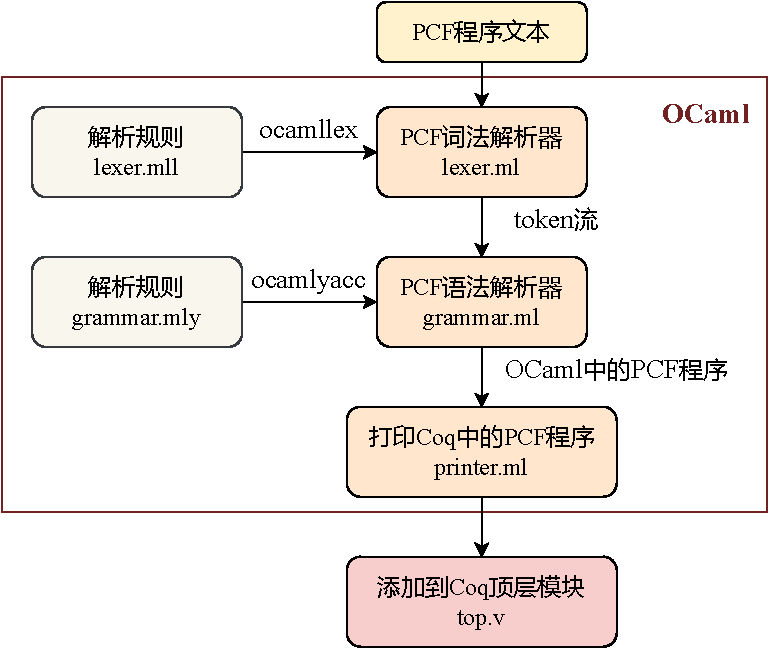
\includegraphics[width=0.7\linewidth]{figures/pcfparser.pdf}
    \caption{PCF语法分析器结构}\label{fig:parser}
\end{figure}

\subsection{程序语言定义}

如上一节所述,我们已经使用PCF语法分析器在Coq顶层编译模块得到了PCF程序的抽象语法树。
除了PCF语言的抽象语法树定义,我们还为其在Coq中实现了第~\ref{sec:cps}节中定义的小步操作语义。
我们使用Inductive类型完成了这种程序状态转换规则的定义。如下代码~\ref{code:pcf}所示,
我们将程序状态用Record类型表示,那么小步操作语义就是pcf\_state类型上的二元关系。
CPS和SSA语言的语法和小步操作语义结构与之类似。不过SSA语言的语法结构和程序状态组成都更加复杂,
在定义小步操作语义时也需要更多的辅助函数,例如由$pc$值获取该位置指令的方法$\mathbf{code}_{at}$等。

\begin{lstlisting}[language=Coq, caption=Coq中的PCF语法与语义定义结构, label=code:pcf]
    Inductive  pcf_term : Set  := ...
    Record  pcf_state  :=  mk_state {t : pcf_term;  ctx : context;}.
    Inductive  pcf_step : pcf_state -> pcf_state -> Prop  := ...
\end{lstlisting}

在编译算法正确性证明过程中使用的小步操作语义是关系型的,即表示为两个程序状态之间的关系。
这样的设计对于证明来说很方便,但是无法在Coq中直接运行某种语言可终止的程序得到返回结果。
在代码实现过程中,为了对操作语义和转换算法进行初步测试,我们在Coq中为PCF、CPS和SSA三种语言分别构建解释器(Interpreter),
从而能够执行相应的程序,得到程序返回的结果。其中,发散的定义要取决于对最大步数的限定,即解释器的\textit{fuel}。
解释器每走一步都会消耗一个\textit{fuel},如果\textit{fuel}消耗完程序还没有终止或出错,就可以认为程序发散了,返回超时状态(Timeout)。
进行解释器测试主要是为了找出操作语义和转换算法中的问题,为接下来的证明减少阻碍。形式化验证过程本身与解释器没有关系。
PCF语言的解释器定义结构如代码~\ref{code:pcfinter}所示。

\begin{lstlisting}[language=Coq, caption=Coq中的PCF语言的解释器, label=code:pcfinter]
    Inductive  pcf_result : Type  := 
        |  terminate : nat  ->  pcf_result 
        |  error : pcf_result
        |  timeout : pcf_result
    Fixpoint  pcf_interpreter  (fuel : nat)  (state : pcf_state) : 
        pcf_result  :=  let  'mk_state  term ctx  :=  state  in
                            match fuel with 
                                | 0  =>  timeout 
                                | S fuel'  =>  match  term, ctx  with ...
\end{lstlisting}

我们为PCF、CPS与SSA语言完成了语法、小步操作语义及解释器在Coq中的实现,就可以开始进行转换算法的实现了。

\subsection{转换算法的实现}

CPS转换算法~\ref{algo:cpstrans}和CPS到SSA的转换算法~\ref{cps2ssa}均在Coq中进行实现。
对于CPS转换,我们需要根据已有的变量名称列表生成新变量,且新变量不能与已有的变量名重复。
在具体实现时,我们采用的算法是为新生成的变量维护一个后缀最大值$n$。
当需要生成一个新的变量名时,我们首先尝试将前缀字符串后连接后缀$n$,并将后缀最大值加一。
这样一个字符串虽然不会与新生成的变量名冲突,但是可能会和CPS程序原有的变量名冲突。
由于我们的CPS转换算法会持续记录已有的变量名列表$l_v$,我们还需要使之与$l_v$中的
变量比较。如果产生冲突,需要重复上一步。
对于CPS到SSA的转换算法,如代码~\ref{code:cpsssa}所示,我们首先需要实现插入指令、
基本代码块、函数的$\mathbf{app}$操作。
然后,我们需要能够根据已处理的条件语句数量$n$生成新的基本代码块标签的操作fresh\_block\_label。
之后,我们就可以实现~\ref{sec:cpsssatrans}节中的转换算法了。

\begin{lstlisting}[language=Coq, caption=Coq中CPS到SSA的转换算法, label=code:cpsssa]  
    Definition  app_i  (i : instruction)  (t : ssa_term)  (p : pc)  : 
        ssa_term  := ... 
    Definition  fresh_block_label  (n : nat)  :  string  := ...
    Definition  G_state  :  Type  :=  (ssa_term  *  nat  *  loc_cps).
    Fixpoint  G  (t_cps : cps_term)  (t_ssa : ssa_term)  (p : pc)  
        (n : nat)  (loc : loc_cps)  :  G_state  := ...
    Definition  G_prog  (t_cps : cps_term)  :  ssa_term  := ...
\end{lstlisting}

我们还实现了从SSA到Vellvm抽象语法树的编译过程。
将Vellvm作为子模块使用,该转换步骤的目标语言是Vellvm在\textit{Syntax.LLVMAst}文件中定义的LLVM IR。
正如我们在介绍SSA语言时所说,该SSA保留了LLVM IR程序的结构。
此步转换主要是进行结构上的映射,顺便为被省略的参数选取正确的默认值。
例如,我们可以直接把SSA中的函数调用指令$x = \mathbf{call}\; f\; v$转换为LLVM AST中的
INSTR\_Op指令,但是需要为其指定$f$和$v$的类型。在这里我们统一使用64位无符号整型。
其他结构同理,基本代码块转换为LLVMAst.block,函数转换为definition,顶层翻译单元转换为toplevel\_entities。
得到Vellvm中的抽象语法树后,就可以利用其提供的工具进行LLVM程序的输出或使用LLVM后续的编译过程了。

\subsection{定理证明的实现} \label{sec:implthm}

完成了程序语言小步操作语义的定义和编译算法的实现,我们就可以对第~\ref{ch:verify}节中
介绍的相关定理进行证明了。
由于两步转换的前向模拟证明结构相似,此处代码~\ref{code:cpsssav}以CPS到SSA的转换为例。

首先,我们需要定义CPS与SSA程序状态之间的不变式match\_state以及度量函数measure。
那么,定理~\ref{trm:simustep2}在Coq中就可以表示为simulation\_step。
我们使用归纳证明(Proof by Induction)的方法对simulation\_step进行证明。
如下方代码所示,我们对CPS程序状态进行一步转换所遵循的小步操作语义规则进行归纳,即Hstep。
这样,我们证明的目标就按照不同的转换规则分成了很多个子目标(Subgoal)。
在每个子目标中,我们可以根据具体的Hstep规则构造出相应的新的SSA程序状态ssa\_state',
并根据已有的假设证明新的CPS程序状态cps\_state'与ssa\_state'仍然满足不变式。
其中,从旧的SSA状态ssa\_state到新状态之间经历的若干步小步操作语义转换规则需要在
证明时具体给出,这样才能保证ssa\_state'是从ssa\_state出发可以到达的状态。

\begin{lstlisting}[language=Coq, caption=Coq中CPS到SSA程序内部执行步骤模拟的证明, label=code:cpsssav]  
    Inductive  match_state  :  cps_state  ->  ssa_state  ->  
        Prop  := ...
    Definition  measure  (state : cps_state)  :  nat  := ...
    Lemma  simulation_step  :
        forall  cps_state  cps_state'  ssa_state,
            cps_step  cps_state  cps_state' ->
            match_state  cps_state  ssa_state ->
        exists  ssa_state',  
            (plus  ssa_step  ssa_state  ssa_state'  \/
            (star  ssa_step  ssa_state  ssa_state'  /\  
                measure  cps_state'  <  measure  cps_state))  /\
            match_state  cps_state'  ssa_state'.          
    Proof.
        ...induction  Hstep;  intros  Sssa Hmatch;  try  (...).
        ...
\end{lstlisting}

完成CPS到SSA转换中程序内部执行步骤模拟的证明后,我们在Coq中定义了CPS和SSA程序的初始状态、可终止
及发散,并完成了前向模拟性质的证明。
将CPS转换与CPS到SSA转换的前向模拟组合起来,我们得到了从PCF到SSA的前向模拟。
为了证明后向模拟性质,我们还需要证明SSA程序的确定性,即定理~\ref{trm:ssadeter}。
以下代码~\ref{code:back}中的定理是为了完成后向模拟性质证明所需要用到的。接下来将对它们进行简要的介绍。
需要特别说明的是,正如在本文第一章中所说,我们不对错误的程序进行讨论。
并且,对于PCF程序,我们只讨论不会卡住的程序,即我们默认PCF源程序不会在一个非终止的状态下
无法进行下一步转换。如果需要对这种性质进行形式化证明,需要使用局部无名表示( Locally Nameless Representation)
的方法替代有名字的变量表示方法。

\begin{itemize}
    \item \textbf{ssa\_step\_determinism:}对于任意一个SSA程序状态state,如果它不是终止状态,
        它经过一步小步操作语义转换到达的下一个状态是确定的。
    \item \textbf{ssa\_terminate\_determinism:}对于任意一个SSA程序t,如果它会终止,
        那么它终止返回的结果值是确定的。
    \item \textbf{pcf\_diverge\_or\_terminate:}对于任意一个PCF程序t,如果它不会卡住,
        即不会在某个非终止的状态无法进行下一步转换,那么它要么终止,要么发散。
    \item \textbf{ssa\_diverge\_or\_terminate:}对于任意一个SSA程序t,它要么终止,要么发散。
    \item \textbf{can\_not\_terminate:}对于任意一个PCF程序pcf\_term,如果它不终止,那么
        由它编译得到的SSA程序ssa\_term也不会终止。
\end{itemize}

\begin{lstlisting}[language=Coq, caption=Coq中后向模拟证明所需的定理, label=code:back]  
    Theorem  ssa_step_determinism:
        forall  state  state1  state2,
        ssa_step  state  state1  ->  ssa_step  state  state2  ->
        state1  =  state2.
    Theorem  ssa_terminate_determinism:
        forall  t  n1  n2,
        ssa_terminate  t  n1  ->  ssa_terminate  t  n2  ->
        n1  =  n2.
    Lemma  pcf_diverge_or_terminate :
        forall  t,
        pcf_not_stuck  t  ->  ~ (pcf_can_terminate  t)  -> 
        pcf_diverge  t.
    Lemma  ssa_diverge_or_terminates:
        forall  t,
        ssa_diverge  t  /\  ssa_can_terminate  t  ->
        False.
    Theorem  can_not_terminate:
        forall  pcf_term  ssa_term,
        pcf_not_stuck  pcf_term  ->  ssa_term  =  comp  pcf_term 
        ->  ~ (pcf_can_terminate  pcf_term)  
        ->  ~ (ssa_can_terminate  ssa_term).
\end{lstlisting}

那么,利用以上定理以及PCF到SSA的正向模拟,即可完成我们需要证明的目标定理~\ref{trm:bterm}和~\ref{trm:bdiv}。
具体的证明过程已在第~\ref{sec:combback}节中进行介绍。
完成了这些证明,就能够说明PCF到SSA编译算法实现了语义保存。

\section{Coq代码评估}

Coq中各主要模块类别和内容的代码行数(Lines of Code, LOC)如表~\ref{tabeval}。
可以看到,相关定理的证明即转换算法验证部分是工作量占比最大的。
我们没有对PCF语法分析器的代码进行LOC评估,因为正如第~\ref{sec:pcfparser}节中所说,
它们是利用ocamllex和ocamlyacc工具生成的。
这里只统计了Coq中从PCF抽象语法树到目标SSA程序抽象语法树的编译与验证代码,它们是根据
本文第\ref{ch:trans}章和第\ref{ch:verify}章的内容实现的。
除了Coq标准库,证明过程中还使用到了CompCert在\textit{common.Smallstep}模块中一步转换关系上的
部分运算与相关定理~\cite{leroy2009formally}。Vellvm抽象语法树的定义以及后续与LLVM IR相关的
工具使用了提供操作语义版本的Vellvm~\cite{vellvm2012}。
这些使用他人工作的子模块代码都没有计入LOC统计。

\begin{table}
    \linespread{1.25}
    \small
    \centering
    % \vspace{-20pt}
    \caption{Coq代码LOC评估}\label{tabeval}
    \begin{center}
    \begin{tabular}{|l|l|l|l|}
    \hline
    代码类别 & 代码实现内容 & LOC & 行数占比(\%) \\
    \hline
    \multirow{3}{*}{程序语言定义} & PCF & 171 & \multirow{3}{*}{23.9} \\
        & CPS & 228 & \\
        & SSA & 303 & \\
        \hline
    \multirow{3}{*}{转换算法} & PCF$\rightarrow$CPS & 148 & \multirow{3}{*}{24.5} \\
        & CPS$\rightarrow$SSA & 251 & \\
        & SSA$\rightarrow$LLVM IR & 318 & \\
        \hline
    \multirow{4}{*}{形式化验证} & PCF$\rightarrow$CPS前向模拟 & 364 & \multirow{4}{*}{51.6} \\
        & CPS$\rightarrow$SSA前向模拟 & 696 & \\
        & 前向模拟组合 & 49 & \\
        & 后向模拟 & 404 & \\
        \hline
    \end{tabular}
    \end{center}
\end{table}


% % !TEX root = ../main.tex

\chapter{数学与引用文献的标注}

\section{数学}

\subsection{数字和单位}

宏包 \pkg{siunitx} 提供了更好的数字和单位支持:
\begin{itemize}
  \item \num{12345.67890}
  \item \complexnum{1+-2i}
  \item \num{.3e45}
  \item \numproduct{1.654 x 2.34 x 3.430}
  \item \unit{kg.m.s^{-1}}
  \item \unit{\micro\meter} $\unit{\micro\meter}$
  \item \unit{\ohm} $\unit{\ohm}$
  \item \numlist{10;20}
  \item \numlist{10;20;30}
  \item \qtylist{0.13;0.67;0.80}{\milli\metre}
  \item \numrange{10}{20}
  \item \qtyrange{10}{20}{\degreeCelsius}
\end{itemize}

\subsection{数学符号和公式}

按照国标 GB/T 3102.11—1993《物理科学和技术中使用的数学符号》,
微分符号 $\dd$ 应使用直立体。除此之外,数学常数也应使用直立体:
\begin{itemize}
  \item 微分符号 $\dd$:\cs{dd}
  \item 圆周率 $\uppi$:\cs{uppi}
  \item 自然对数的底 $\ee$:\cs{ee}
  \item 虚数单位 $\ii$, $\jj$:\cs{ii} \cs{jj}
\end{itemize}

公式应另起一行居中排版。公式后应注明编号,按章顺序编排,编号右端对齐。
\begin{equation}
  \ee^{\ii\uppi} + 1 = 0,
\end{equation}
\begin{equation}
  \frac{\dd^2 u}{\dd t^2} = \int f(x) \dd x.
\end{equation}

公式末尾是需要添加标点符号的,至于用逗号还是句号,取决于公式下面一句是接着公式说的,还是另起一句。
\begin{equation}
  \frac{2h}{\pi}\int_{0}^{\infty}\frac{\sin\left( \omega\delta \right)}{\omega}
  \cos\left( \omega x \right) \dd\omega = 
  \begin{cases}
    h, & \left| x \right| < \delta, \\
    \frac{h}{2}, & x = \pm \delta, \\
    0, & \left| x \right| > \delta.
  \end{cases}
\end{equation}
公式较长时最好在等号“$=$”处转行。
\begin{align}
    & I (X_3; X_4) - I (X_3; X_4 \mid X_1) - I (X_3; X_4 \mid X_2) \nonumber \\
  = & [I (X_3; X_4) - I (X_3; X_4 \mid X_1)] - I (X_3; X_4 \mid \tilde{X}_2) \\
  = & I (X_1; X_3; X_4) - I (X_3; X_4 \mid \tilde{X}_2).
\end{align}

如果在等号处转行难以实现,也可在 $+$、$-$、$\times$、$\div$ 运算符号处转行,转行
时运算符号仅书写于转行式前,不重复书写。
\begin{multline}
  \frac{1}{2} \Delta (f_{ij} f^{ij}) =
    2 \left(\sum_{i<j} \chi_{ij}(\sigma_{i} - \sigma_{j})^{2}
    + f^{ij} \nabla_{j} \nabla_{i} (\Delta f) \right. \\
  \left. + \nabla_{k} f_{ij} \nabla^{k} f^{ij} +
    f^{ij} f^{k} \left[2\nabla_{i}R_{jk}
    - \nabla_{k} R_{ij} \right] \vphantom{\sum_{i<j}} \right).
\end{multline}

\subsection{定理环境}

示例文件中使用 \pkg{ntheorem} 宏包配置了定理、引理和证明等环境。用户也可以使用
\pkg{amsthm} 宏包。

这里举一个“定理”和“证明”的例子。
\begin{theorem}[留数定理]
\label{thm:res}
  假设 $U$ 是复平面上的一个单连通开子集,$a_1, \ldots, a_n$ 是复平面上有限个点,
  $f$ 是定义在 $U \backslash \{a_1, \ldots, a_n\}$ 上的全纯函数,如果 $\gamma$
  是一条把 $a_1, \ldots, a_n$ 包围起来的可求长曲线,但不经过任何一个 $a_k$,并且
  其起点与终点重合,那么:

  \begin{equation}
    \label{eq:res}
    \oint\limits_\gamma f(z)\, \dd z = 2\uppi \ii \sum_{k=1}^n \operatorname{I}(\gamma, a_k) \operatorname{Res}(f, a_k).
  \end{equation}

  如果 $\gamma$ 是若尔当曲线,那么 $\operatorname{I}(\gamma, a_k) = 1$,因此:

  \begin{equation}
    \label{eq:resthm}
    \oint\limits_\gamma f(z)\, \dd z = 2\uppi \ii \sum_{k=1}^n \operatorname{Res}(f, a_k).
  \end{equation}

  在这里,$\operatorname{Res}(f, a_k)$ 表示 $f$ 在点 $a_k$ 的留数,
  $\operatorname{I}(\gamma, a_k)$ 表示 $\gamma$ 关于点 $a_k$ 的卷绕数。卷绕数是
  一个整数,它描述了曲线 $\gamma$ 绕过点 $a_k$ 的次数。如果 $\gamma$ 依逆时针方
  向绕着 $a_k$ 移动,卷绕数就是一个正数,如果 $\gamma$ 根本不绕过 $a_k$,卷绕数
  就是零。

  定理~\ref{thm:res} 的证明。

  \begin{proof}
    首先,由……

    其次,……

    所以……
  \end{proof}
\end{theorem}

\section{引用文献的标注}

按照教务处的要求,参考文献外观应符合国标 GB/T 7714 的要求。模版使用 \BibLaTeX{}
配合 \pkg{biblatex-gb7714-2015} 样式包%
\footnote{\url{https://www.ctan.org/pkg/biblatex-gb7714-2015}}%
控制参考文献的输出样式,后端采用 \pkg{biber} 管理文献。

请注意 \pkg{biblatex-gb7714-2015} 宏包 2016 年 9 月才加入 CTAN,如果你使用的
\TeX{} 系统版本较旧,可能没有包含 \pkg{biblatex-gb7714-2015} 宏包,需要手动安装。
\BibLaTeX{} 与 \pkg{biblatex-gb7714-2015} 目前在活跃地更新,为避免一些兼容性问
题,推荐使用较新的版本。

正文中引用参考文献时,使用 \verb|\cite{key1,key2,key3...}| 可以产生“上标引用的参
考文献”,如 \cite{Yu2001,Cheng1999,LSC1957}。使用
\verb|\parencite{key1,key2,key3...}| 则可以产生水平引用的参考文献,例如
\parencite{Li1999,Jiang1989,Hopkinson1999}。请看下面的例子,将会穿插使用水平的和
上标的参考文献:普通图书\parencite{Yu2001,Jiang1998},论文集、会议录
\cite{CSTAM1990},科技报告\parencite{WHO1970},学位论文\cite{Zhang1998},专利文
献\parencite{Jiang1989,HBLZ2001},专著中析出的文献\cite{Cheng1999,GBT2659},期刊
中析出的文献\parencite{Li1999,Li2000},报纸中析出的文献\cite{Ding2000}, 电子文献
\parencite{Jiang1999,Christine1998,Xiao2001}。

可以使用 \verb|\nocite{key1,key2,key3...}| 将参考文献条目加入到文献表中但不在正
文中引用。使用 \verb|\nocite{*}| 可以将参考文献数据库中的所有条目加入到文献表
中。
\nocite{Yang1999,Schinstock2000,Wen1990,GBT16159}

% % !TeX root = ../main.tex

\chapter{浮动体}

\section{插图}

插图功能是利用 \TeX{} 的特定编译程序提供的机制实现的,不同的编译程序支持不同的图
形方式。有的同学可能听说“\LaTeX{} 只支持 EPS”,事实上这种说法是不准确的。\XeTeX{}
可以很方便地插入 EPS、PDF、PNG、JPEG 格式的图片。

一般图形都是处在浮动环境中。之所以称为浮动是指最终排版效果图形的位置不一定与源文
件中的位置对应,这也是刚使用 \LaTeX{} 同学可能遇到的问题。如果要强制固定浮动图形
的位置,请使用 \pkg{float} 宏包,它提供了 \texttt{[H]} 参数。

\subsection{单个图形}

图要有图题,研究生图题采用中英文对照,并置于图的编号之后,图的编号和图题应置于图
下方的居中位置。引用图应在图题右上角标出文献来源。当插图中组成部件由数字或字母等
编号表示时,可在插图下方添加图注进行说明,如图~\ref{fig:cn_100t} 所示。

\begin{figure}[!htp]
  \centering
  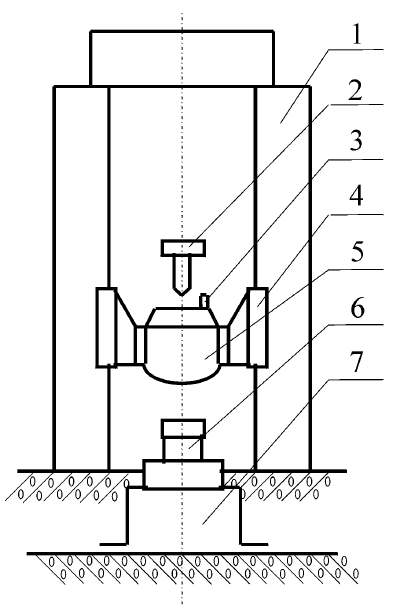
\includegraphics[width=4cm]{cn_100t.png} \\
    1.立柱 2.提升释放机构 3.标准冲击加速度计 \\
    4.导轨 5.重锤 6.被校力传感器 7.底座 \\
  \bicaption[出现在插图索引中]
    {单个图形示例\cite{He1999}。如果表格的标题很长,那么在表格索引中就会很不美观。可
      以在前面用中括号写一个简短的标题,这个标题会出现在索引中。}
    {Stay hungry, stay foolish.}
  \label{fig:cn_100t}
\end{figure}

\subsection{多个图形}

简单插入多个图形的例子如图~\ref{fig:SRR} 所示。这两个水平并列放置的子图共用一个
图形计数器,没有各自的子图题。

\begin{figure}[!htp]
  \centering
  
\includegraphics[height=2cm]{sjtu-vi-badge-blue.pdf}
  \hspace{1cm}
  
\includegraphics[height=2cm]{sjtu-vi-badge-blue.pdf}
  \bicaption{中文题图}{English caption}
  \label{fig:SRR}
\end{figure}

如果多个图形相互独立,并不共用一个图形计数器,那么用 \texttt{minipage} 或者
\texttt{parbox} 就可以,如图~\ref{fig:parallel1} 与图~\ref{fig:parallel2}。

\begin{figure}[!htp]
  \centering
  \begin{minipage}{0.48\textwidth}
    \centering
    
\includegraphics[height=1.5cm]{sjtu-vi-name-blue.pdf}
    \caption{并排第一个图}
    \label{fig:parallel1}
  \end{minipage}\hfill
  \begin{minipage}{0.48\textwidth}
    \centering
    
\includegraphics[height=1.5cm]{sjtu-vi-name-blue.pdf}
    \caption{并排第二个图}
    \label{fig:parallel2}
  \end{minipage}
\end{figure}

如果要为共用一个计数器的多个子图添加子图题,建议使用较新的 \pkg{subcaption}宏
包,不建议使用 \pkg{subfigure} 或 \pkg{subfig} 等宏包。

推荐使用 \pkg{subcaption} 宏包的 \cs{subcaptionbox} 并排子图,子图题置于子图之
下,子图号用 a)、b) 等表示。也可以使用 \pkg{subcaption} 宏包的 \cs{subcaption}
(放在 minipage中,用法同 \cs{caption})。

\pkg{subcaption} 宏包也提供了 \pkg{subfigure} 和 \pkg{subtable} 环境,如
图~\ref{fig:subfigure}。

\begin{figure}[!htp]
  \centering
  \begin{subfigure}{0.3\textwidth}
    \centering
    
\includegraphics[height=2cm]{sjtu-vi-badge-blue.pdf}
    \caption{校徽}
  \end{subfigure}
  \hspace{1cm}
  \begin{subfigure}{0.4\textwidth}
    \centering
    
\includegraphics[height=1.5cm]{sjtu-vi-name-blue.pdf}
    \caption{校名。注意这个图略矮些,subfigure 中同一行的子图在顶端对齐。}
  \end{subfigure}
  \caption{包含子图题的范例(使用 subfigure)}
  \label{fig:subfigure}
\end{figure}

搭配 \pkg{bicaption} 宏包时,可以启用 \cs{subcaptionbox} 和 \cs{subcaption} 的双
语变种 \cs{bisubcaptionbox} 和 \cs{bisubcaption},如图~\ref{fig:bisubcaptionbox}
所示。

\begin{figure}[!hbtp]
  \centering
  \bisubcaptionbox{$R_3 = 1.5\text{mm}$ 时轴承的压力分布云图}%
                  {Pressure contour of bearing when $R_3 = 1.5\text{mm}$}%
                  [6.4cm]{\includegraphics[height=3cm]{example-image-a.pdf}}
  \hspace{1cm}
  \bisubcaptionbox{$R_3 = 2.5\text{mm}$ 时轴承的压力分布云图}%
                  {Pressure contour of bearing when $R_3 = 2.5\text{mm}$}%
                  [6.4cm]{\includegraphics[height=3cm]{example-image-b.pdf}}
  \bicaption{包含子图题的范例(使用 subcaptionbox)}
            {Example with subcaptionbox}
  \label{fig:bisubcaptionbox}
\end{figure}


\section{表格}

\subsection{基本表格}

编排表格应简单明了,表达一致,明晰易懂,表文呼应、内容一致。表题置于表上,研究生
学位论文可以用中、英文两种文字居中排写,中文在上,也可以只用中文。

表格的编排建议采用国际通行的三线表\footnote{三线表,以其形式简洁、功能分明、阅读
方便而在科技论文中被推荐使用。三线表通常只有 3 条线,即顶线、底线和栏目线,没有
竖线。}。三线表可以使用 \pkg{booktabs} 提供的 \cs{toprule}、\cs{midrule} 和
\cs{bottomrule}。它们与 \pkg{longtable} 能很好的配合使用。

\begin{table}[!hpt]
  \caption[一个颇为标准的三线表]{一个颇为标准的三线表\footnotemark}
  \label{tab:firstone}
  \centering
  \begin{tabular}{@{}llr@{}} \toprule
    \multicolumn{2}{c}{Item} \\ \cmidrule(r){1-2}
    Animal & Description & Price (\$)\\ \midrule
    Gnat  & per gram  & 13.65 \\
          & each      & 0.01 \\
    Gnu   & stuffed   & 92.50 \\
    Emu   & stuffed   & 33.33 \\
    Armadillo & frozen & 8.99 \\ \bottomrule
  \end{tabular}
\end{table}
\footnotetext{这个例子来自
  \href{https://mirrors.sjtug.sjtu.edu.cn/ctan/macros/latex/contrib/booktabs/booktabs.pdf}%
  {《Publication quality tables in LaTeX》}(\pkg{booktabs} 宏包的文档)。这也是
  一个在表格中使用脚注的例子,请留意与 \pkg{threeparttable} 实现的效果有何不
  同。}

\subsection{复杂表格}

我们经常会在表格下方标注数据来源,或者对表格里面的条目进行解释。可以用
\pkg{threeparttable} 实现带有脚注的表格,如表~\ref{tab:footnote}。

\begin{table}[!htpb]
  \bicaption{一个带有脚注的表格的例子}{A Table with footnotes}
  \label{tab:footnote}
  \centering
  \begin{threeparttable}[b]
     \begin{tabular}{ccd{4}cccc}
      \toprule
      \multirow{2}*{total} & \multicolumn{2}{c}{20\tnote{a}} & \multicolumn{2}{c}{40} & \multicolumn{2}{c}{60} \\
      \cmidrule(lr){2-3}\cmidrule(lr){4-5}\cmidrule(lr){6-7}
      & www & \multicolumn{1}{c}{k} & www & k & www & k \\ % 使用说明符 d 的列会自动进入数学模式,使用 \multicolumn 对文字表头做特殊处理
      \midrule
      & $\underset{(2.12)}{4.22}$ & 120.0140\tnote{b} & 333.15 & 0.0411 & 444.99 & 0.1387 \\
      & 168.6123 & 10.86 & 255.37 & 0.0353 & 376.14 & 0.1058 \\
      & 6.761    & 0.007 & 235.37 & 0.0267 & 348.66 & 0.1010 \\
      \bottomrule
    \end{tabular}
    \begin{tablenotes}
    \item [a] the first note.
    \item [b] the second note.
    \end{tablenotes}
  \end{threeparttable}
\end{table}

如某个表需要转页接排,可以用 \pkg{longtable} 实现。接排时表题省略,表头应重复书
写,并在右上方写“续表 xx”,如表~\ref{tab:performance}。

\begin{ThreePartTable}
  \begin{TableNotes}
    \item[a] 一个脚注
    \item[b] 另一个脚注
  \end{TableNotes}
  \begin{longtable}[c]{c*{6}{r}}
    \bicaption{实验数据}{Experimental data}
    \label{tab:performance} \\
    \toprule
    测试程序 & \multicolumn{1}{c}{正常运行} & \multicolumn{1}{c}{同步}
      & \multicolumn{1}{c}{检查点} & \multicolumn{1}{c}{卷回恢复}
      & \multicolumn{1}{c}{进程迁移} & \multicolumn{1}{c}{检查点} \\
    & \multicolumn{1}{c}{时间 (s)} & \multicolumn{1}{c}{时间 (s)}
      & \multicolumn{1}{c}{时间 (s)} & \multicolumn{1}{c}{时间 (s)}
      & \multicolumn{1}{c}{时间 (s)} &  文件(KB)\\
    \midrule
    \endfirsthead
    \multicolumn{7}{l}{\textbf{续表~\thetable}} \\
    % 英语论文:\multicolumn{7}{r}{\textbf{Table~\thetable~(continued)}} \\
    \toprule
    测试程序 & \multicolumn{1}{c}{正常运行} & \multicolumn{1}{c}{同步}
      & \multicolumn{1}{c}{检查点} & \multicolumn{1}{c}{卷回恢复}
      & \multicolumn{1}{c}{进程迁移} & \multicolumn{1}{c}{检查点} \\
    & \multicolumn{1}{c}{时间 (s)} & \multicolumn{1}{c}{时间 (s)}
      & \multicolumn{1}{c}{时间 (s)} & \multicolumn{1}{c}{时间 (s)}
      & \multicolumn{1}{c}{时间 (s)}&  文件(KB)\\
    \midrule
    \endhead
    \hline
    \multicolumn{7}{r}{续下页}
    \endfoot
    \insertTableNotes
    \endlastfoot
    CG.A.2 & 23.05 & 0.002 & 0.116 & 0.035 & 0.589 & 32491 \\
    CG.A.4 & 15.06 & 0.003 & 0.067 & 0.021 & 0.351 & 18211 \\
    CG.A.8 & 13.38 & 0.004 & 0.072 & 0.023 & 0.210 & 9890 \\
    CG.B.2 & 867.45 & 0.002 & 0.864 & 0.232 & 3.256 & 228562 \\
    CG.B.4 & 501.61 & 0.003 & 0.438 & 0.136 & 2.075 & 123862 \\
    CG.B.8 & 384.65 & 0.004 & 0.457 & 0.108 & 1.235 & 63777 \\
    MG.A.2 & 112.27 & 0.002 & 0.846 & 0.237 & 3.930 & 236473 \\
    MG.A.4 & 59.84 & 0.003 & 0.442 & 0.128 & 2.070 & 123875 \\
    MG.A.8 & 31.38 & 0.003 & 0.476 & 0.114 & 1.041 & 60627 \\
    MG.B.2 & 526.28 & 0.002 & 0.821 & 0.238 & 4.176 & 236635 \\
    MG.B.4 & 280.11 & 0.003 & 0.432 & 0.130 & 1.706 & 123793 \\
    MG.B.8 & 148.29 & 0.003 & 0.442 & 0.116 & 0.893 & 60600 \\
    LU.A.2 & 2116.54 & 0.002 & 0.110 & 0.030 & 0.532 & 28754 \\
    LU.A.4 & 1102.50 & 0.002 & 0.069 & 0.017 & 0.255 & 14915 \\
    LU.A.8 & 574.47 & 0.003 & 0.067 & 0.016 & 0.192 & 8655 \\
    LU.B.2 & 9712.87 & 0.002 & 0.357 & 0.104 & 1.734 & 101975 \\
    LU.B.4 & 4757.80 & 0.003 & 0.190 & 0.056 & 0.808 & 53522 \\
    LU.B.8 & 2444.05 & 0.004 & 0.222 & 0.057 & 0.548 & 30134 \\
    EP.A.2 & 123.81 & 0.002 & 0.010 & 0.003 & 0.074 & 1834 \\
    EP.A.4 & 61.92 & 0.003 & 0.011 & 0.004 & 0.073 & 1743 \\
    EP.A.8 & 31.06 & 0.004 & 0.017 & 0.005 & 0.073 & 1661 \\
    EP.B.2 & 495.49 & 0.001 & 0.009 & 0.003 & 0.196 & 2011 \\
    EP.B.4 & 247.69 & 0.002 & 0.012 & 0.004 & 0.122 & 1663 \\
    EP.B.8 & 126.74 & 0.003 & 0.017 & 0.005 & 0.083 & 1656 \\
    SP.A.2 & 123.81 & 0.002 & 0.010 & 0.003 & 0.074 & 1854 \\
    SP.A.4 & 51.92 & 0.003 & 0.011 & 0.004 & 0.073 & 1543 \\
    SP.A.8 & 31.06 & 0.004 & 0.017 & 0.005 & 0.073 & 1671 \\
    SP.B.2 & 495.49 & 0.001 & 0.009 & 0.003 & 0.196 & 2411 \\
    SP.B.4 \tnote{a} & 247.69 & 0.002 & 0.014 & 0.006 & 0.152 & 2653 \\
    SP.B.8 \tnote{b} & 126.74 & 0.003 & 0.017 & 0.005 & 0.082 & 1755 \\
    \bottomrule
  \end{longtable}
\end{ThreePartTable}

\section{算法环境}

算法环境可以使用 \pkg{algorithms} 宏包或者较新的 \pkg{algorithm2e} 实现。
算法~\ref{algo:algorithm} 是一个使用 \pkg{algorithm2e} 的例子。关于排版算法环境
的具体方法,请阅读相关宏包的官方文档。

\begin{algorithm}[htb]
  \caption{算法示例}
  \label{algo:algorithm}
  \small
  \SetAlgoLined
  \KwData{this text}
  \KwResult{how to write algorithm with \LaTeXe }

  initialization\;
  \While{not at end of this document}{
    read current\;
    \eIf{understand}{
      go to next section\;
      current section becomes this one\;
    }{
      go back to the beginning of current section\;
    }
  }
\end{algorithm}

\section{代码环境}

我们可以在论文中插入算法,但是不建议插入大段的代码。如果确实需要插入代码,建议使
用 \pkg{listings} 宏包。

\begin{codeblock}[language=C]
#include <stdio.h>
#include <unistd.h>
#include <sys/types.h>
#include <sys/wait.h>

int main() {
  pid_t pid;

  switch ((pid = fork())) {
  case -1:
    printf("fork failed\n");
    break;
  case 0:
    /* child calls exec */
    execl("/bin/ls", "ls", "-l", (char*)0);
    printf("execl failed\n");
    break;
  default:
    /* parent uses wait to suspend execution until child finishes */
    wait((int*)0);
    printf("is completed\n");
    break;
  }

  return 0;
}
\end{codeblock}

% !TEX root = ../main.tex

\chapter{全文总结} \label{ch:summary}

\section{主要结论}

\section{研究展望}


%TC:ignore

% 参考文献
\printbibliography[heading=bibintoc]

% 附录
\appendix

% 附录中图表不加入索引
\captionsetup{list=no}

% 附录内容
% % !TEX root = ../main.tex

\chapter{Maxwell Equations}

选择二维情况,有如下的偏振矢量:
\begin{subequations}
  \begin{align}
    {\bf E} &= E_z(r, \theta) \hat{\bf z}, \\
    {\bf H} &= H_r(r, \theta) \hat{\bf r} + H_\theta(r, \theta) \hat{\bm\theta}.
  \end{align}
\end{subequations}
对上式求旋度:
\begin{subequations}
  \begin{align}
    \nabla \times {\bf E} &= \frac{1}{r} \frac{\partial E_z}{\partial\theta}
      \hat{\bf r} - \frac{\partial E_z}{\partial r} \hat{\bm\theta}, \\
    \nabla \times {\bf H} &= \left[\frac{1}{r} \frac{\partial}{\partial r}
      (r H_\theta) - \frac{1}{r} \frac{\partial H_r}{\partial\theta} \right]
      \hat{\bf z}.
  \end{align}
\end{subequations}
因为在柱坐标系下,$\overline{\overline\mu}$ 是对角的,所以 Maxwell 方程组中电场
$\bf E$ 的旋度:
\begin{subequations}
  \begin{align}
    & \nabla \times {\bf E} = \ii \omega {\bf B}, \\
    & \frac{1}{r} \frac{\partial E_z}{\partial\theta} \hat{\bf r} -
      \frac{\partial E_z}{\partial r}\hat{\bm\theta} = \ii \omega \mu_r H_r
      \hat{\bf r} + \ii \omega \mu_\theta H_\theta \hat{\bm\theta}.
  \end{align}
\end{subequations}
所以 $\bf H$ 的各个分量可以写为:
\begin{subequations}
  \begin{align}
    H_r &= \frac{1}{\ii \omega \mu_r} \frac{1}{r}
      \frac{\partial E_z}{\partial\theta}, \\
    H_\theta &= -\frac{1}{\ii \omega \mu_\theta}
      \frac{\partial E_z}{\partial r}.
  \end{align}
\end{subequations}
同样地,在柱坐标系下,$\overline{\overline\epsilon}$ 是对角的,所以 Maxwell 方程
组中磁场 $\bf H$ 的旋度:
\begin{subequations}
  \begin{align}
    & \nabla \times {\bf H} = -\ii \omega {\bf D}, \\
    & \left[\frac{1}{r} \frac{\partial}{\partial r}(r H_\theta) - \frac{1}{r}
      \frac{\partial H_r}{\partial\theta} \right] \hat{\bf z} = -\ii \omega
      {\overline{\overline\epsilon}} {\bf E} = -\ii \omega \epsilon_z E_z
      \hat{\bf z}, \\
    & \frac{1}{r} \frac{\partial}{\partial r}(r H_\theta) - \frac{1}{r}
      \frac{\partial H_r}{\partial\theta} = -\ii \omega \epsilon_z E_z.
  \end{align}
\end{subequations}
由此我们可以得到关于 $E_z$ 的波函数方程:
\begin{equation}
  \frac{1}{\mu_\theta \epsilon_z} \frac{1}{r} \frac{\partial}{\partial r}
  \left(r \frac{\partial E_z}{\partial r} \right) + \frac{1}{\mu_r \epsilon_z}
  \frac{1}{r^2} \frac{\partial^2E_z}{\partial\theta^2} +\omega^2 E_z = 0.
\end{equation}

% % !TEX root = ../main.tex

\chapter{绘制流程图}

图~\ref{fig:flow_chart} 是一张流程图示意。使用 \pkg{tikz} 环境,搭配四种预定义节
点(\verb|startstop|、\verb|process|、\verb|decision| 和 \verb|io|),可以容易地
绘制出流程图。

\begin{figure}[!htp]
  \centering
  
% 定义流程图节点
\tikzstyle{startstop} = [
  rectangle,
  rounded corners,
  minimum width=4em,
  text centered,
  inner sep=1.5ex,
  draw
]
\tikzstyle{io} = [
  trapezium,
  trapezium left angle=75,
  trapezium right angle=105,
  minimum width=4em,
  text centered,
  inner sep=1.5ex,
  draw
]
\tikzstyle{process} = [
  rectangle,
  minimum width=4em,
  text centered,
  inner sep=1.5ex,
  draw
]
\tikzstyle{decision} = [
  diamond,
  minimum width=4em,
  aspect=2,
  text centered,
  draw
]
\tikzstyle{arrow} = [-{LaTeX}]

\begin{tikzpicture}[node distance=1.5cm, every node/.style={font=\footnotesize}]
  % 设置节点
  \node[startstop] (pic) {待测图片};
  \node[io, below of=pic] (bg) {读取背景};
  \node[process, below of=bg] (pair) {匹配特征点对};
  \node[decision, below of=pair, yshift=-2ex] (threshold) {多于阈值};
  \node[decision, right of=threshold, xshift=3cm] (clear) {清晰?};
  \node[process, right of=pair, xshift=3cm] (capture) {重采};
  \node[process, below of=threshold, yshift=-2ex] (matrix_p) {透视变换矩阵};
  \node[process, right of=matrix_p, xshift=3cm] (matrix_a) {仿射变换矩阵};
  \node[process, below of=matrix_p] (reg) {图像修正};
  \node[startstop, below of=reg] (return) {配准结果};
    
  % 连接节点
  \draw[arrow] (pic) -- (bg);
  \draw[arrow] (bg) -- (pair);
  \draw[arrow] (pair) -- (threshold);

  \draw[arrow] (threshold) -- node[above] {否} (clear);

  \draw[arrow] (clear) -- node[right] {否} (capture);
  \draw[arrow] (capture) |- (pic);
  \draw[arrow] (clear) -- node[right] {是} (matrix_a);
  \draw[arrow] (matrix_a) |- (reg);

  \draw[arrow] (threshold) -- node[left] {是} (matrix_p);
  \draw[arrow] (matrix_p) -- (reg);
  \draw[arrow] (reg) -- (return);
\end{tikzpicture}

  \bicaption{绘制流程图效果}{Flow chart}
  \label{fig:flow_chart}
\end{figure}


% 结尾部分
\backmatter

% 用于盲审的论文需隐去致谢、发表论文、科研成果、简历

% 致谢
% !TEX root = ../main.tex

\begin{acknowledgements}
  感谢那位最先制作出博士学位论文 \LaTeX{} 模板的物理系同学!

  感谢 William Wang 同学对模板移植做出的贡献!

  感谢 \href{https://github.com/weijianwen}{@weijianwen} 学长开创性的工作!

  感谢 \href{https://github.com/sjtug}{@sjtug} 对 0.10 及之后版本的开发和维护工作!

  感谢所有为模板贡献过代码的\href{https://github.com/sjtug/SJTUThesis/graphs/contributors}{同学们}, 以及所有测试和使用模板的各位同学!

  感谢 \LaTeX 和 \href{https://github.com/sjtug/SJTUThesis}{SJTUThesis},帮我节省了不少时间。
\end{acknowledgements}


% 发表论文及科研成果
% 盲审论文中,发表论文及科研成果等仅以第几作者注明即可,不要出现作者或他人姓名
% !TEX root = ../main.tex

\begin{achievements}

\subsection*{学术论文}

% 明审版
\begin{bibliolist}{00}
  \item Siyu Liu and Yuting Wang. Verified Transformation of Continuation-Passing 
    Style into Static Single Assignment Form. 
    In Theoretical Aspects of Software Engineering (TASE), 2023: 20–37. 
\end{bibliolist}

% 盲审版
\begin{bibliolist*}{00}
  \item Theoretical Aspects of Software Engineering (TASE)会议(CCF-C类)文章,第一作者, 2023.
\end{bibliolist*}

\end{achievements}


% 简历
% % !TEX root = ../main.tex

\begin{resume}
  \subsection*{基本情况}
    某某,yyyy 年 mm 月生于 xxxx。

  \subsection*{教育背景}
  \begin{itemize}
    \item yyyy 年 mm 月至今,上海交通大学,博士研究生,xx 专业
    \item yyyy 年 mm 月至 yyyy 年 mm 月,上海交通大学,硕士研究生,xx 专业
    \item yyyy 年 mm 月至 yyyy 年 mm 月,上海交通大学,本科,xx 专业
  \end{itemize}

  \subsection*{研究兴趣}
    \LaTeX{} 排版

  \subsection*{联系方式}
  \begin{itemize}
    \item 地址: 上海市闵行区东川路 800 号,200240
    \item E-mail: \email{john_smith@sjtu.edu.cn}
  \end{itemize}
\end{resume}


% 学士学位论文要求在最后有一个大摘要,单独编页码
% % !TEX root = ../main.tex

\begin{digest}
  An imperial edict issued in 1896 by Emperor Guangxu, established Nanyang
  Public School in Shanghai. The normal school, school of foreign studies,
  middle school and a high school were established. Sheng Xuanhuai, the person
  responsible for proposing the idea to the emperor, became the first president
  and is regarded as the founder of the university.

  During the 1930s, the university gained a reputation of nurturing top
  engineers. After the foundation of People's Republic, some faculties were
  transferred to other universities. A significant amount of its faculty were
  sent in 1956, by the national government, to Xi'an to help build up Xi'an Jiao
  Tong University in western China. Afterwards, the school was officially
  renamed Shanghai Jiao Tong University.

  Since the reform and opening up policy in China, SJTU has taken the lead in
  management reform of institutions for higher education, regaining its vigor
  and vitality with an unprecedented momentum of growth. SJTU includes five
  beautiful campuses, Xuhui, Minhang, Luwan Qibao, and Fahua, taking up an area
  of about \qty{3225833}{\square\metre}. A number of disciplines have been
  advancing towards the top echelon internationally, and a batch of burgeoning
  branches of learning have taken an important position domestically.

  Today SJTU has 31 schools (departments), 63 undergraduate programs, 250
  masters-degree programs, 203 Ph.D. programs, 28 post-doctorate programs, and
  11 state key laboratories and national engineering research centers.

  SJTU boasts a large number of famous scientists and professors, including 35
  academics of the Academy of Sciences and Academy of Engineering, 95 accredited
  professors and chair professors of the ``Cheung Kong Scholars Program'' and
  more than \num{2000} professors and associate professors.

  Its total enrollment of students amounts to \num{35929}, of which \num{1564}
  are international students. There are \num{16802} undergraduates, and
  \num{17563} masters and Ph.D. candidates. After more than a century of
  operation, Jiao Tong University has inherited the old tradition of ``high
  starting points, solid foundation, strict requirements and extensive
  practice.'' Students from SJTU have won top prizes in various competitions,
  including ACM International Collegiate Programming Contest, International
  Mathematical Contest in Modeling and Electronics Design Contests. Famous
  alumni include Jiang Zemin, Lu Dingyi, Ding Guangen, Wang Daohan, Qian Xuesen,
  Wu Wenjun, Zou Taofen, Mao Yisheng, Cai Er, Huang Yanpei, Shao Lizi, Wang An
  and many more. More than 200 of the academics of the Chinese Academy of
  Sciences and Chinese Academy of Engineering are alumni of Jiao Tong
  University.
\end{digest}


%TC:endignore

\end{document}
